%%
%% Cow Pi Datasheet (c) 2021-22 Christopher A. Bohn
%%
%% Licensed under the Apache License, Version 2.0 (the "License");
%% you may not use this file except in compliance with the License.
%% You may obtain a copy of the License at
%%     http://www.apache.org/licenses/LICENSE-2.0
%% Unless required by applicable law or agreed to in writing, software
%% distributed under the License is distributed on an "AS IS" BASIS,
%% WITHOUT WARRANTIES OR CONDITIONS OF ANY KIND, either express or implied.
%% See the License for the specific language governing permissions and
%% limitations under the License.
%%

\documentclass[12pt]{article}

\usepackage{amsmath}
\usepackage{amssymb}
\usepackage[letterpaper, margin=1in]{geometry}
\usepackage{etoolbox}
\usepackage{fancyhdr}
\usepackage{graphicx}
\usepackage{hyperref}
\usepackage[procnames]{listings}
\usepackage{setspace}
\usepackage{subfig}
\usepackage{textcomp}
\usepackage{tikz}
\usetikzlibrary{shapes.geometric}
\usepackage{xcolor}

\lstset{language=C, tabsize=4, upquote=true, basicstyle=\ttfamily, numberstyle=\color{gray}, numbers=left, showspaces=false, showstringspaces=false}
\newcommand{\function}[1]{\textbf{\lstinline{#1}}}
\newcommand{\functionitem}[3]{\item \hypertarget{function:#2}{\lstinline{#1} \function{#2} \lstinline{(#3)}}\addcontentsline{toc}{subsubsection}{\function{#2}}}
\hypersetup{colorlinks=true}

%! suppress = NonMatchingIf
\newcommand{\hardwareversion}{unknown}
\newcommand{\construction}{unknown}
\newcommand{\mcuboard}{unknown}
\newcommand{\photograph}{unknown}
\newcommand{\microcontroller}{unknown}
\newcommand{\displaymoduledescription}{unknown}

\providebool{spi}
\providebool{i2c}
\providebool{max7219digits}
\providebool{max7219matrix}
\providebool{lcd1602}
\providebool{nano-form-factor}
\providebool{pico-form-factor}

\ifdefstring{\cowpiversion}{mk1c}{
    \renewcommand{\hardwareversion}{mark~1c}
    \renewcommand{\construction}{solderless breadboard}
    \renewcommand{\mcuboard}{Arduino Nano}
    \setbool{spi}{true}
    \setbool{max7219digits}{true}
    \renewcommand{\photograph}{../hardware/mk1a.jpg}    % close enough
}{}

\ifdefstring{\cowpiversion}{mk1d}{
    \renewcommand{\hardwareversion}{mark~1d}
    \renewcommand{\construction}{solderless breadboard}
    \renewcommand{\mcuboard}{Arduino Nano}
    \setbool{i2c}{true}
    \setbool{lcd1602}{true}
    \renewcommand{\photograph}{../hardware/mk1d.jpg}
}{}

\ifdefstring{\cowpiversion}{mk3a}{
    \renewcommand{\hardwareversion}{mark~3a}
    \renewcommand{\construction}{through-hole printed circuit board}
    \renewcommand{\mcuboard}{Arduino Nano}
    \setbool{spi}{true}
    \setbool{i2c}{true}
    \setbool{lcd1602}{true}
    \renewcommand{\photograph}{../hardware/mk3a.jpg}
}{}


\ifdefstring{\mcuboard}{Arduino Nano}{
    \renewcommand{\microcontroller}{ATmega328P}
    \setbool{nano-form-factor}{true}
}{}
\ifboolexpe{bool{max7219digits}}{\renewcommand{\displaymoduledescription}{8-digit 7-segment LED display}}{}
\ifboolexpe{bool{max7219matrix}}{\renewcommand{\displaymoduledescription}{$8 \times 8$ LED matrix display}}{}
\ifboolexpe{bool{lcd1602}}{\renewcommand{\displaymoduledescription}{$2 \times 16$ LCD dot-matrix character display}}{}

\begin{document}
    \pagestyle{fancy}
    \fancyhf{}
    \lhead{Cow Pi \cowpiversion\ Development Board}
    \rhead{CowPi v\softwareversion\ Library}
    \cfoot{\thepage}
    \title{Cow Pi, \hardwareversion\footnote{The Cow Pi hardware design, library, example code, and documentation \copyright 2021--22, Christopher A. Bohn}}
    \author{Datasheet}
    \date{}
    \maketitle

    The \hardwareversion\ Cow Pi is a member of the Cow Pi product line from Eclectic Electronics\footnote{
        Eclectic Electronics is a joint subsidiary of The Pleistocene Petting Zoo, a Limited-Reality Corporation, and of Babbage's Analytic Engines, a Frankly-Figmentary Partnership.}
    and is guaranteed to bring you minutes of fun.
    Whether you need a 4-function calculator to count your terror bird eggs before they hatch, an electronic combination lock to secure your wildly-dangerous experimental robots, or a motion alarm to protect yourself from zombie gourds, using the Cow Pi development board is your best option.

    This document describes the use of the Cow Pi \cowpiversion\ development board with the CowPi v\softwareversion\ library.

    \tableofcontents


    \section{Hardware Overview} %! suppress = NonMatchingIf

This section describes the \hardwareversion\ Cow Pi development board, describes the theory of operation for its components, and summarizes the features of its display module.

\subsection{Cow Pi Development Board}

The Cow Pi development board consists of a microcontroller board (\mcuboard), a display module (\displaymoduledescription), a $4 \times 4$ matrix keypad, two momentary buttons, two toggleable switches, and two LEDs.
The board is assembled on a \construction; see Figure~\ref{fig:photograph}.

%! suppress = FileNotFound
\begin{figure}
    \centering
    \includegraphics[scale=0.75]{\photograph}
    \caption{A \hardwareversion\ Cow Pi development board.}\label{fig:photograph}
\end{figure}

The toggleable switches are referred to as the \textbf{left switch} and the \textbf{right switch}, and each can be positioned in the left or right position.
When a switch is in the right position, its logic value is high, by way of a pull-up resistor.
When a switch is in the left position, the switch is grounded, and its logic value is low.

The momentary buttons are referred to as the \textbf{left button} and the \textbf{right button}, and each can be pressed (alternatively, in the down position) or unpressed (alternatively, in the up position).
The buttons are normally-open, and so when a button is unpressed, its logic value is high, by way of a pull-up resistor.
When a button is pressed, the button is grounded, and its logic value is low.

The LEDs are referred to as the \textbf{left LED} and the \textbf{right LED}.
\ifboolexpe{bool{nano-form-factor}}{
    The \textbf{left LED} is aliased to the \mcuboard's built-in LED, and some documents may refer to it as the Cow Pi's \textbf{internal LED}.
    \ifdefstring{\construction}{solderless breadboard}{
        Indeed, Arduino-based mark~1 Cow Pis simply use the \mcuboard's built-in LED as the \textbf{left LED} to reduce clutter on the solderless breadboard.
    }{}
    \ifboolexpe{bool{spi}}{
        Note that the \textbf{left LED} may be of limited use in the Cow Pi \cowpiversion\ due to the \mcuboard's \texttt{D13} pin being used for both the \textbf{left} (built-in) \textbf{LED} and also as for the \texttt{SCK} SPI clock signal.
    }{}
    Some documents may refer to the \textbf{right LED} as the Cow Pi's \textbf{external LED}.
}{}
An LED will illuminate when the corresponding microcontroller output is high, and it will deluminate when the corresponding microcontroller output is low.

The matrix keypad is designed to be scanned using the conventional approach of selectively setting the rows' logic values and reading the columns' resulting logic values.
\ifdefstring{\construction}{solderless breadboard}{Note that mark~1 Cow Pis' keypads cannot be accurately scanned if more than two keys are pressed at the same time.
    Further, \textbf{there are no current-limiting protections} (other than the microcontroller's fuses) in place to prevent over-current if simultaneously pressing more than one in the same column shorts a logic-high row to a logic-low row.}{}

The microcontroller communicates with the \displaymoduledescription display module using the
\ifboolexpe{bool{spi}}{Serial Peripheral Interface (SPI) protocol.}{}
\ifboolexpe{bool{i2c}}{Inter-Integrated Circuit (I$^2$C or IIC) protocol, also known as the Two-Wire Interface (TWI) protocol.}{}

\ifboolexpe{bool{spi}}{\ifboolexpe{bool{i2c}}{Figures~\ref{fig:pinouts-nano-spi} and~\ref{fig:pinouts-nano-i2c} show}{Figure~\ref{fig:pinouts-nano-spi} shows}}{\ifboolexpe{bool{i2c}}{Figure~\ref{fig:pinouts-nano-i2c} shows}{}}
which input or output is connected to each of the \mcuboard's pins, as well as which general-purpose input/output register bit corresponds to each pin.

\ifboolexpe{bool{spi}}{
    \begin{figure}[p]
        \centering
        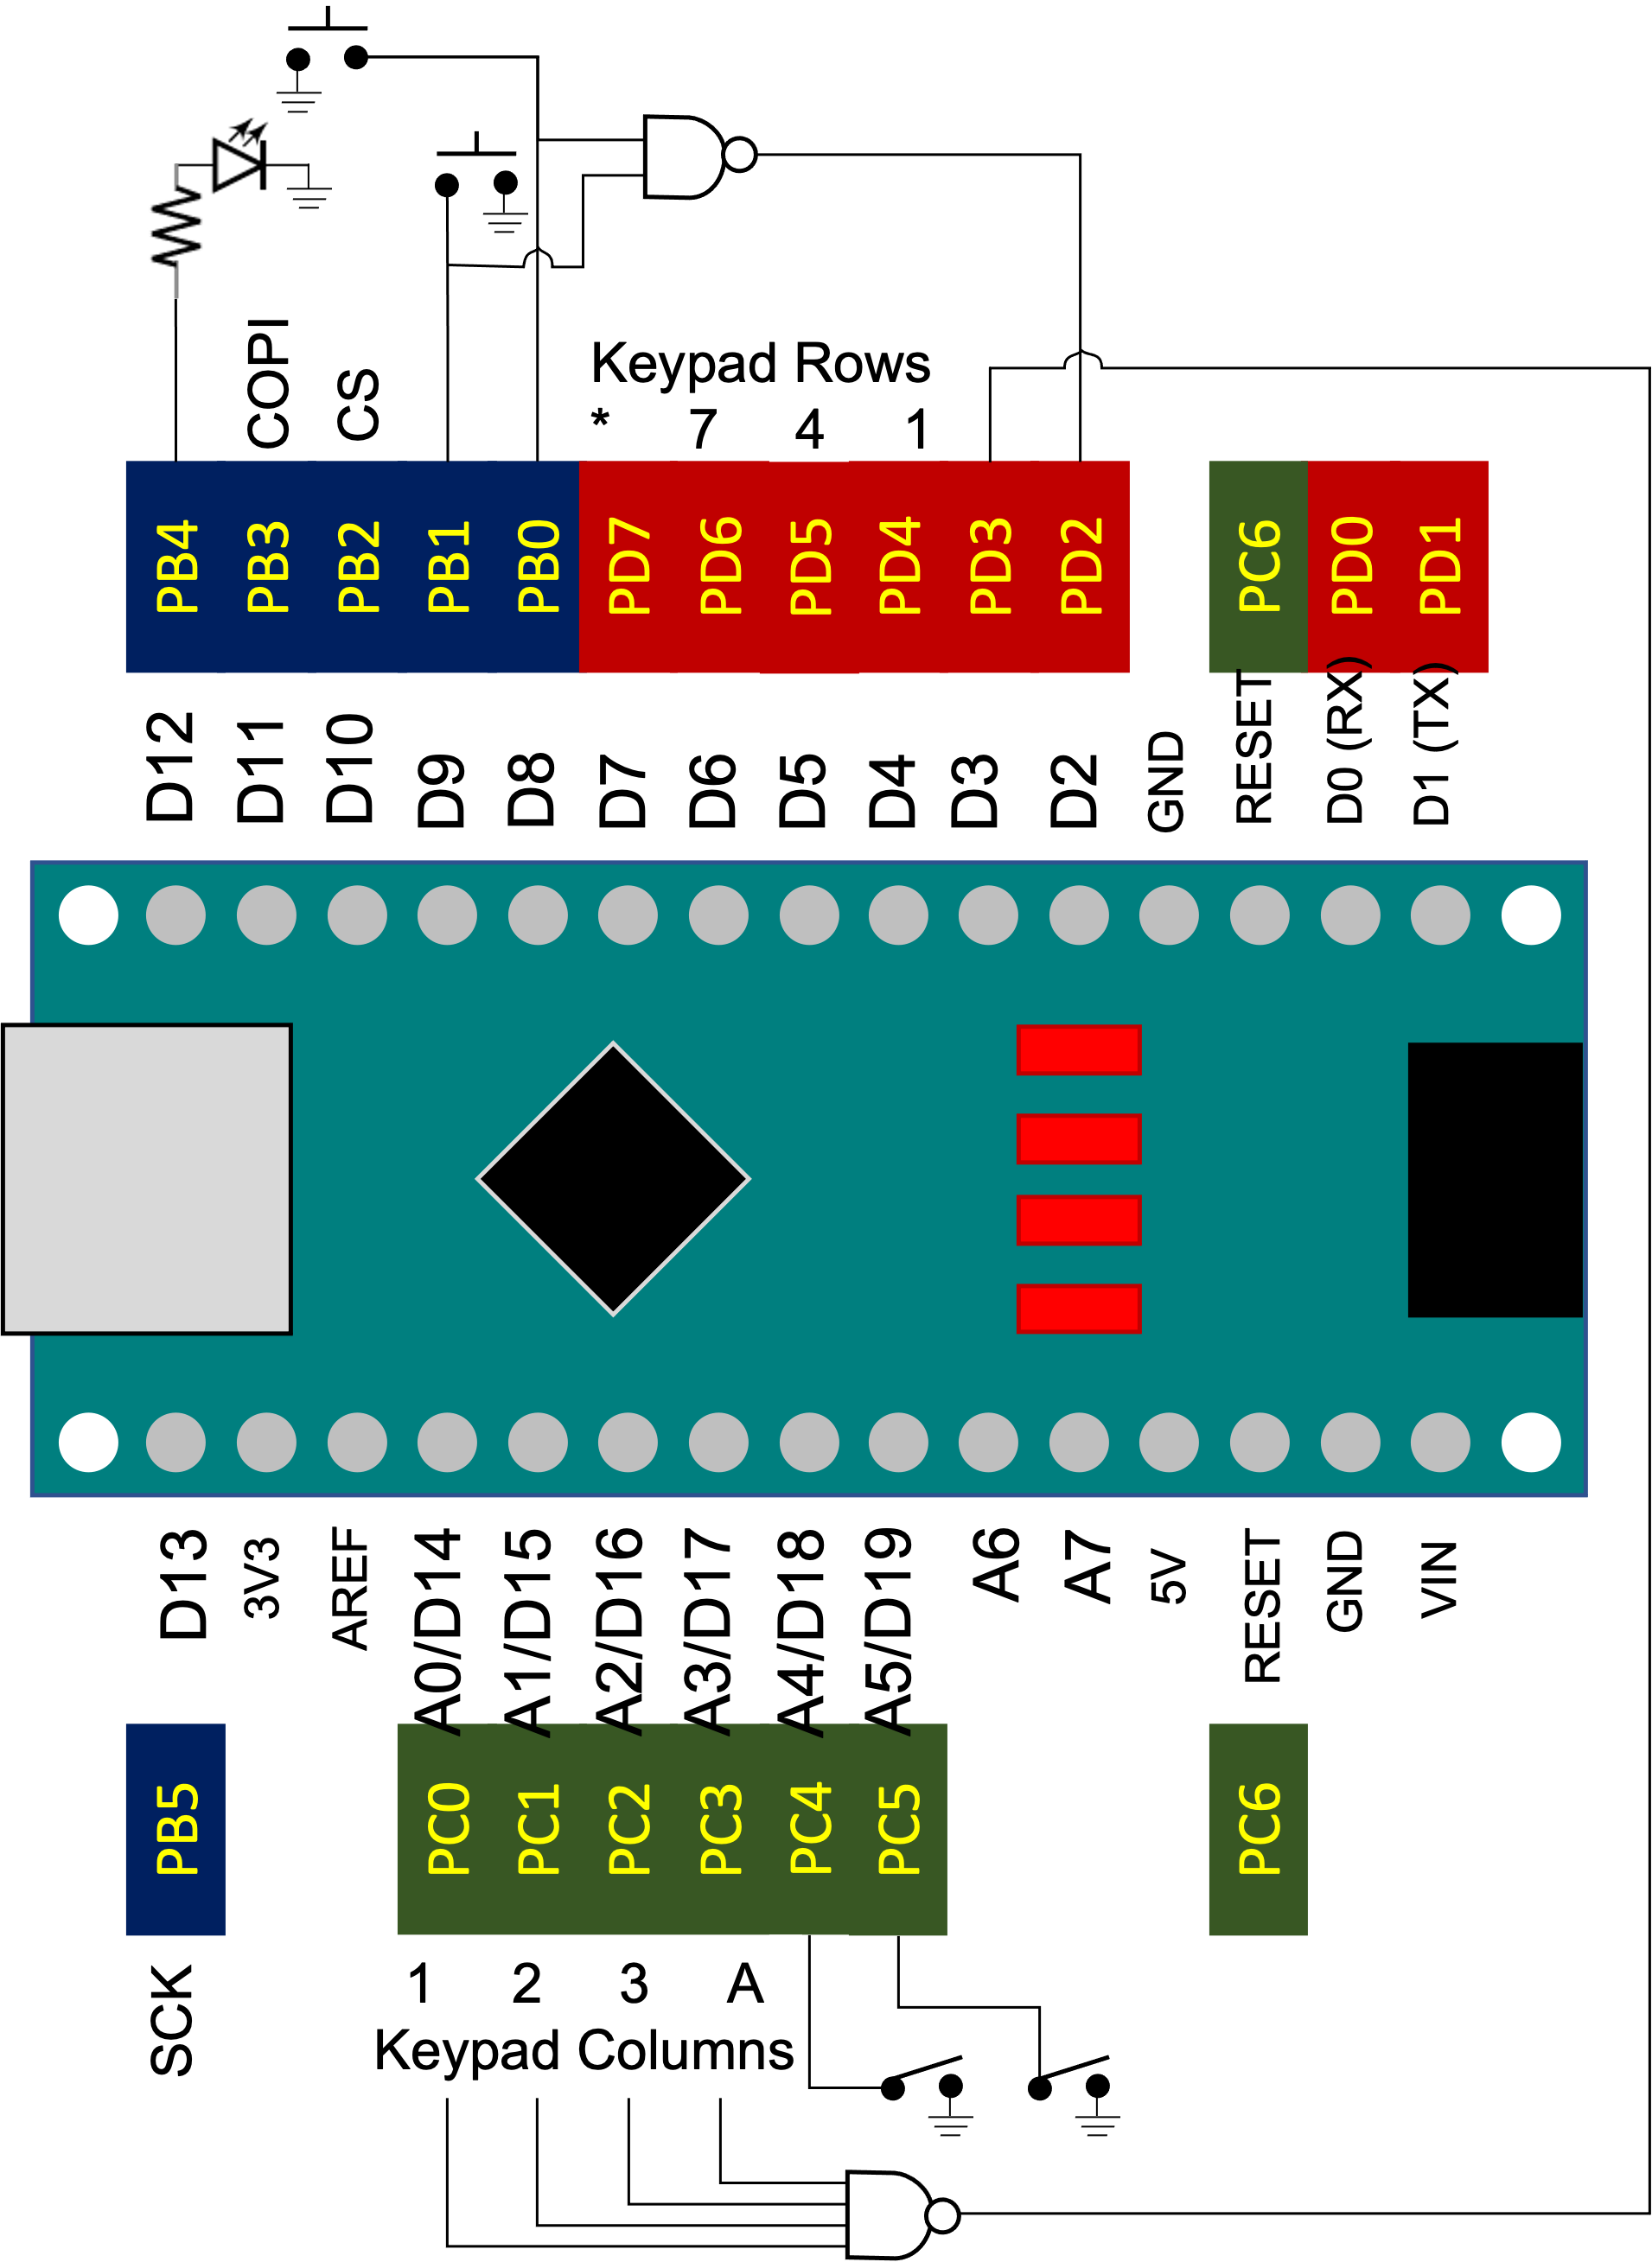
\includegraphics[scale=0.75]{pinouts/nano-spi}
        \caption{Pinout for the \hardwareversion\ Cow Pi development board using \mcuboard and the SPI serial communication protocol.}\label{fig:pinouts-nano-spi}
    \end{figure}
}{}

\ifboolexpe{bool{i2c}}{
    \begin{figure}[p]
        \centering
        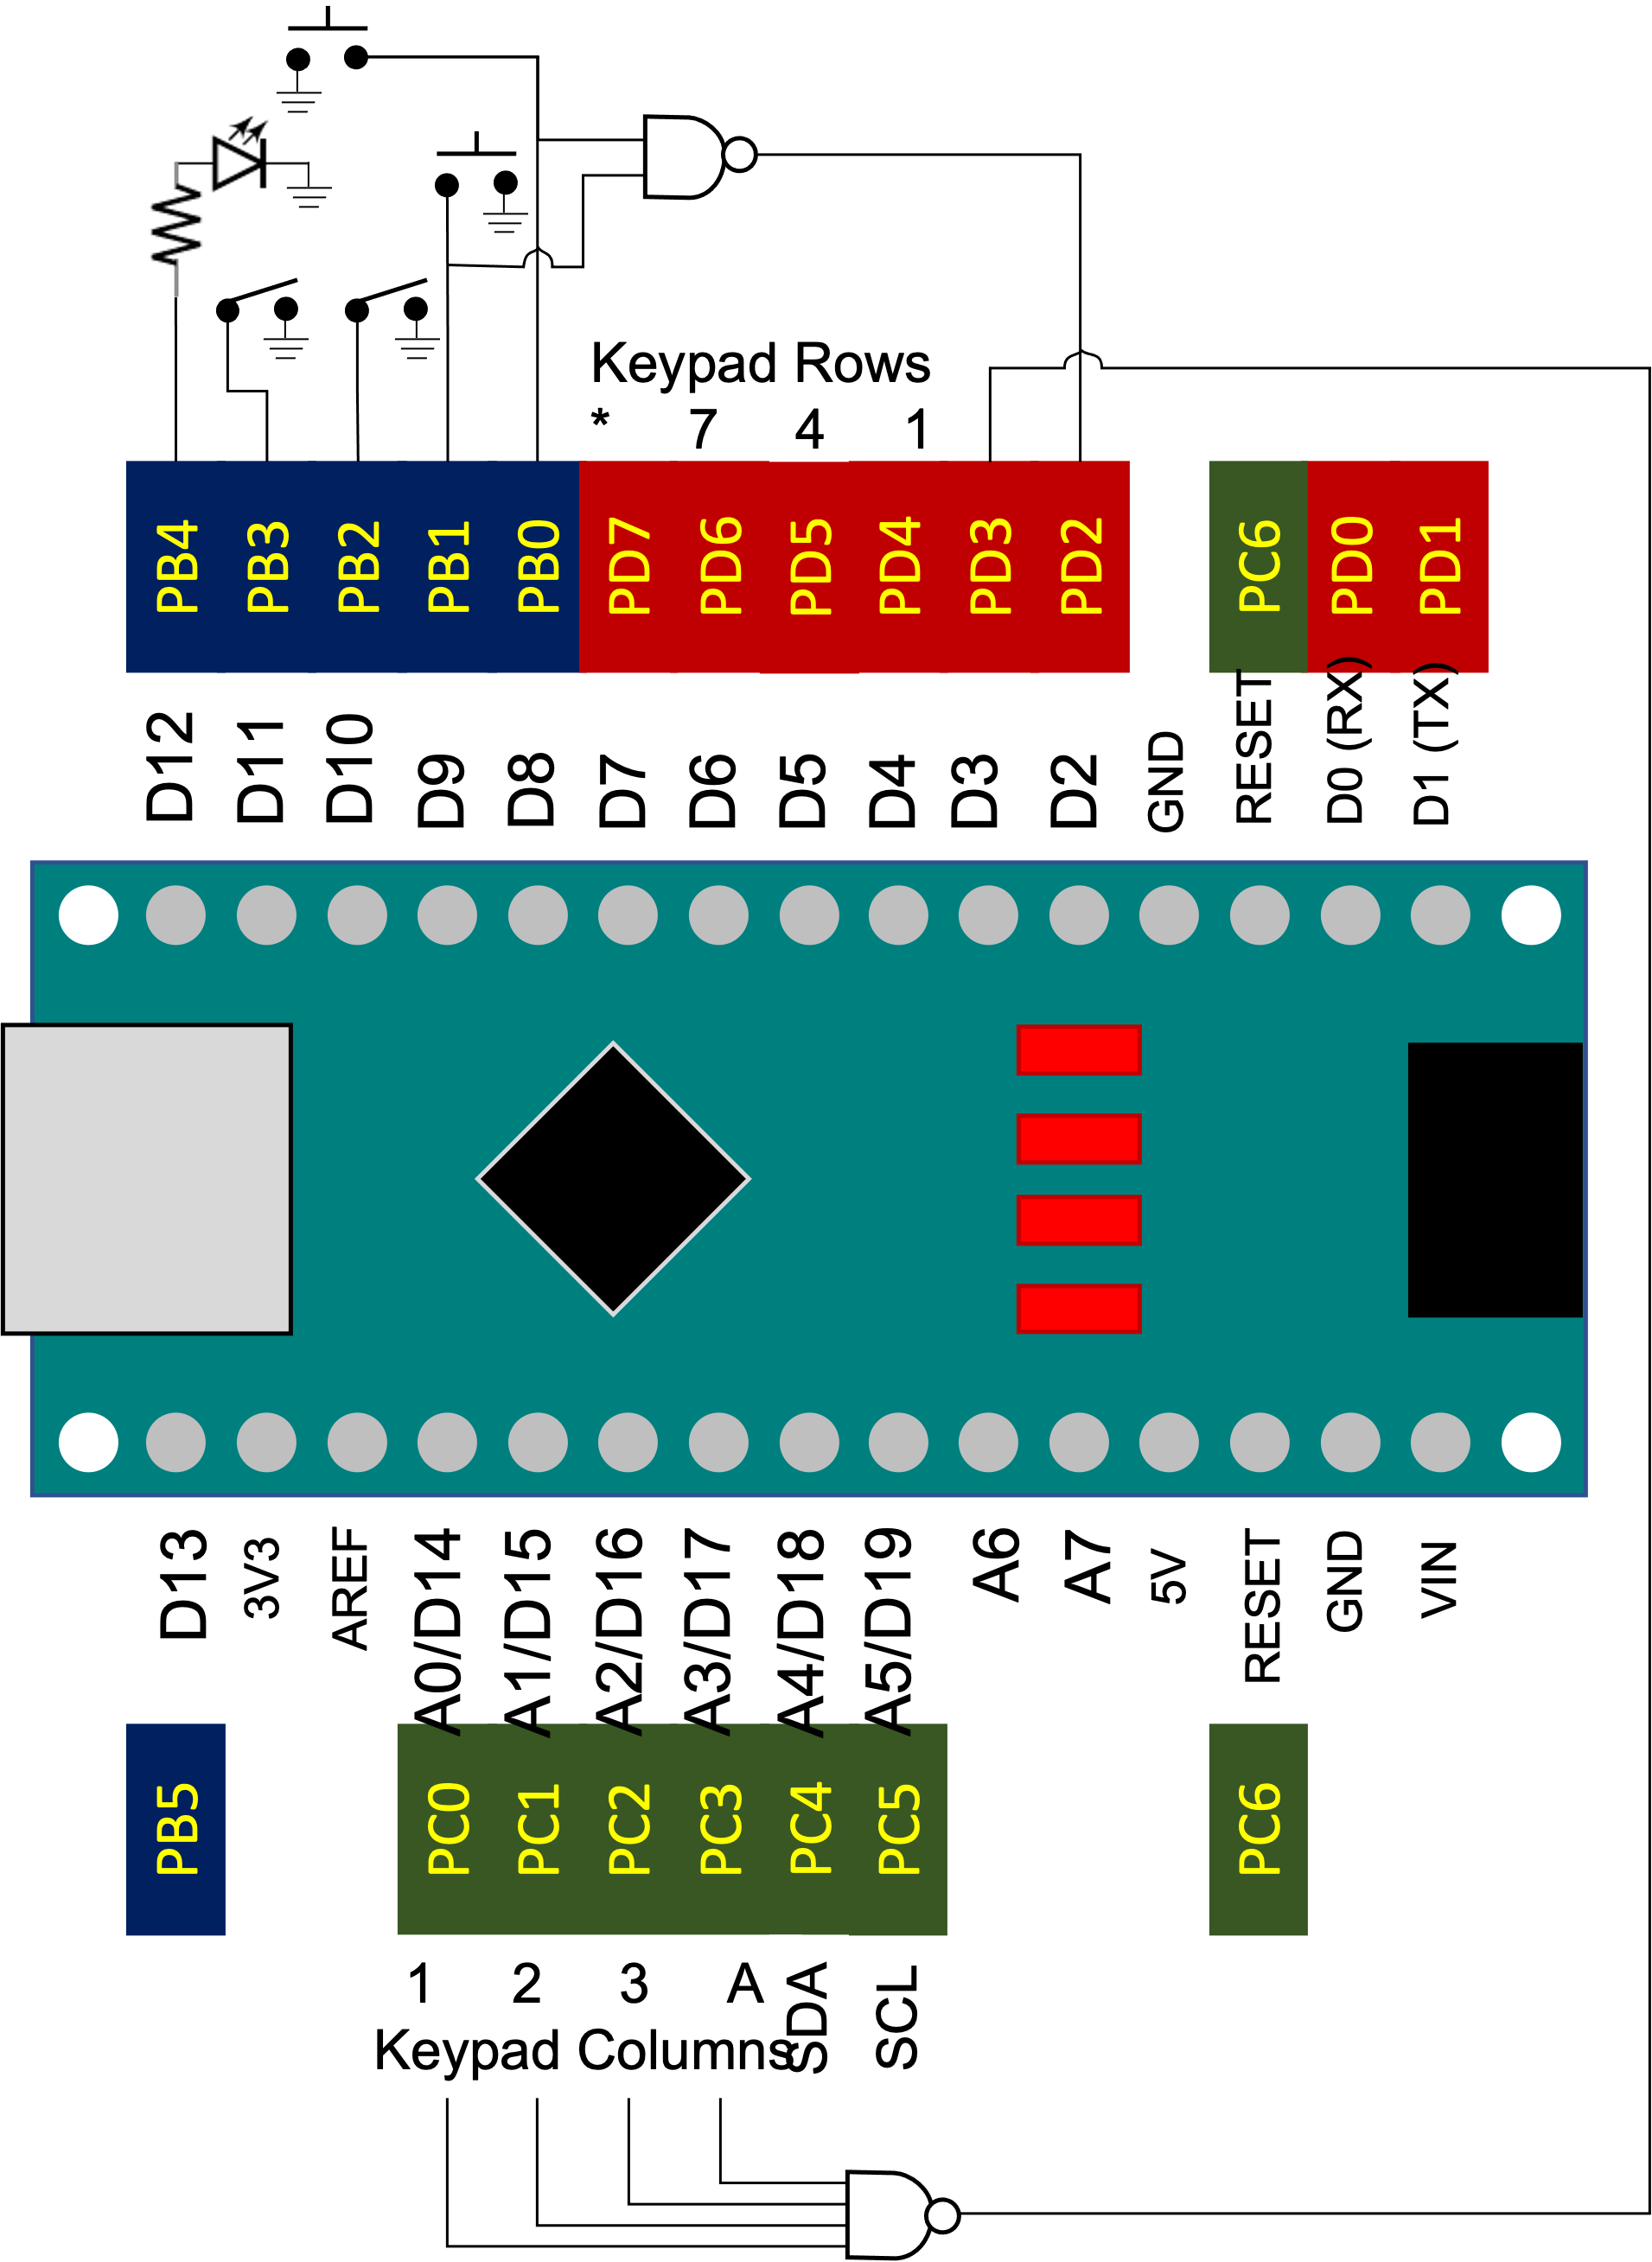
\includegraphics[scale=0.75]{pinouts/nano-i2c}
        \caption{Pinout for a Cow Pi development board using the \mcuboard\ and the I$^2$C serial communication protocol.}\label{fig:pinouts-nano-i2c}
    \end{figure}
}{}

%\subsection{Microcontroller Board}
%
%\subsection{LEDs}
%
%\subsection{Buttons and Switches}
%
\subsection{Matrix Keypad}

\subsubsection{Theory of Operation}

Each key on a matrix keypad is a normally-open, momentary button that resides at the intersection of a row and a column;
see Figure~\ref{fig:basic-keypad}(a).
When pressed, the key closes an electrical connection between that row and column.
On the Cow Pi, each row is connected to an output pin on the \mcuboard, and each column is connected to an input pin with a pull-up resistor.

Because the input pins that the columns are connected to use pull-up resistors, the logic value on these pins will normally read high (boolean 1).
A column will read as logic low (boolean 0) only when it is electrically connected to a row that is set low.
An application developer can take advantage of this by setting all of the rows' pins to logic low (boolean 0);
see Figure~\ref{fig:basic-keypad}(b).
When a key is pressed, its column will then become low.

\begin{figure}[h]
    \hspace{.5in}
    \subfloat[Each key on the keypad is at the intersection of a row and a column.]{
        \centering
        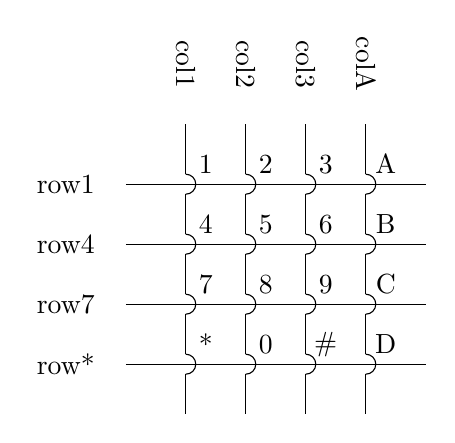
\begin{tikzpicture}[x=.1in, y=.1in]
            \draw (7,10) node {1} +(3,0) node {2} +(6,0) node {3} +(9,0) node {A}
                +(0,-3) node {4} +(3,-3) node {5} +(6,-3) node {6} +(9,-3) node {B}
                +(0,-6) node {7} +(3,-6) node {8} +(6,-6) node {9} +(9,-6) node {C}
                +(0,-9) node {*} +(3,-9) node {0} +(6,-9) node {\#} +(9,-9) node {D};
            \draw (0,9) node {row1} ++(3,0) -- ++(15,0);
            \draw (0,6) node {row4} ++(3,0) -- ++(15,0);
            \draw (0,3) node {row7} ++(3,0) -- ++(15,0);
            \draw (0,0) node {row*} ++(3,0) -- ++(15,0);
            \draw (6,15) node {\rotatebox{-90}{col1}} ++(0,-3) -- ++(0,-2.5) ++(0,-1) -- ++(0,-2) ++(0,-1) -- ++(0,-2) ++(0,-1) -- ++(0,-2) ++(0,-1) -- ++(0,-2);
            \draw (6,9.5) arc [start angle=90, end angle=-90, radius=.5] ++(0,-2) arc [start angle=90, end angle=-90, radius=.5] ++(0,-2) arc [start angle=90, end angle=-90, radius=.5] ++(0,-2) arc [start angle=90, end angle=-90, radius=.5];
            \draw (9,15) node {\rotatebox{-90}{col2}} ++(0,-3) -- ++(0,-2.5) ++(0,-1) -- ++(0,-2) ++(0,-1) -- ++(0,-2) ++(0,-1) -- ++(0,-2) ++(0,-1) -- ++(0,-2);
            \draw (9,9.5) arc [start angle=90, end angle=-90, radius=.5] ++(0,-2) arc [start angle=90, end angle=-90, radius=.5] ++(0,-2) arc [start angle=90, end angle=-90, radius=.5] ++(0,-2) arc [start angle=90, end angle=-90, radius=.5];
            \draw (12,15) node {\rotatebox{-90}{col3}} ++(0,-3) -- ++(0,-2.5) ++(0,-1) -- ++(0,-2) ++(0,-1) -- ++(0,-2) ++(0,-1) -- ++(0,-2) ++(0,-1) -- ++(0,-2);
            \draw (12,9.5) arc [start angle=90, end angle=-90, radius=.5] ++(0,-2) arc [start angle=90, end angle=-90, radius=.5] ++(0,-2) arc [start angle=90, end angle=-90, radius=.5] ++(0,-2) arc [start angle=90, end angle=-90, radius=.5];
            \draw (15,15) node {\rotatebox{-90}{colA}} ++(0,-3) -- ++(0,-2.5) ++(0,-1) -- ++(0,-2) ++(0,-1) -- ++(0,-2) ++(0,-1) -- ++(0,-2) ++(0,-1) -- ++(0,-2);
            \draw (15,9.5) arc [start angle=90, end angle=-90, radius=.5] ++(0,-2) arc [start angle=90, end angle=-90, radius=.5] ++(0,-2) arc [start angle=90, end angle=-90, radius=.5] ++(0,-2) arc [start angle=90, end angle=-90, radius=.5];
        \end{tikzpicture}
    }
    \hfill
    \subfloat[Detecting a keypress is possible by setting each row low and monitoring whether any column becomes low.]{
        \centering
        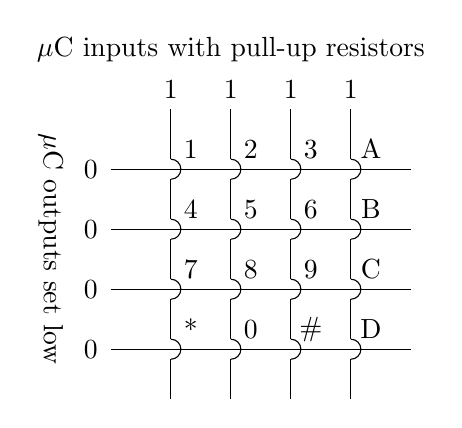
\begin{tikzpicture}[x=.1in, y=.1in]
            \draw (7,10) node {1} +(3,0) node {2} +(6,0) node {3} +(9,0) node {A}
            +(0,-3) node {4} +(3,-3) node {5} +(6,-3) node {6} +(9,-3) node {B}
            +(0,-6) node {7} +(3,-6) node {8} +(6,-6) node {9} +(9,-6) node {C}
            +(0,-9) node {*} +(3,-9) node {0} +(6,-9) node {\#} +(9,-9) node {D};
            \draw (0,5) node {\rotatebox{-90}{$\mu$C outputs set low}};
            \draw (0,9) +(2,0) node {0} ++(3,0) -- ++(15,0);
            \draw (0,6) +(2,0) node {0} ++(3,0) -- ++(15,0);
            \draw (0,3) +(2,0) node {0} ++(3,0) -- ++(15,0);
            \draw (0,0) +(2,0) node {0} ++(3,0) -- ++(15,0);
            \draw (9,15) node {$\mu$C inputs with pull-up resistors};
            \draw (6,15) +(0,-2) node {1} ++(0,-3) -- ++(0,-2.5) ++(0,-1) -- ++(0,-2) ++(0,-1) -- ++(0,-2) ++(0,-1) -- ++(0,-2) ++(0,-1) -- ++(0,-2);
            \draw (6,9.5) arc [start angle=90, end angle=-90, radius=.5] ++(0,-2) arc [start angle=90, end angle=-90, radius=.5] ++(0,-2) arc [start angle=90, end angle=-90, radius=.5] ++(0,-2) arc [start angle=90, end angle=-90, radius=.5];
            \draw (9,15) +(0,-2) node {1} ++(0,-3) -- ++(0,-2.5) ++(0,-1) -- ++(0,-2) ++(0,-1) -- ++(0,-2) ++(0,-1) -- ++(0,-2) ++(0,-1) -- ++(0,-2);
            \draw (9,9.5) arc [start angle=90, end angle=-90, radius=.5] ++(0,-2) arc [start angle=90, end angle=-90, radius=.5] ++(0,-2) arc [start angle=90, end angle=-90, radius=.5] ++(0,-2) arc [start angle=90, end angle=-90, radius=.5];
            \draw (12,15) +(0,-2) node {1} ++(0,-3) -- ++(0,-2.5) ++(0,-1) -- ++(0,-2) ++(0,-1) -- ++(0,-2) ++(0,-1) -- ++(0,-2) ++(0,-1) -- ++(0,-2);
            \draw (12,9.5) arc [start angle=90, end angle=-90, radius=.5] ++(0,-2) arc [start angle=90, end angle=-90, radius=.5] ++(0,-2) arc [start angle=90, end angle=-90, radius=.5] ++(0,-2) arc [start angle=90, end angle=-90, radius=.5];
            \draw (15,15) +(0,-2) node {1} ++(0,-3) -- ++(0,-2.5) ++(0,-1) -- ++(0,-2) ++(0,-1) -- ++(0,-2) ++(0,-1) -- ++(0,-2) ++(0,-1) -- ++(0,-2);
            \draw (15,9.5) arc [start angle=90, end angle=-90, radius=.5] ++(0,-2) arc [start angle=90, end angle=-90, radius=.5] ++(0,-2) arc [start angle=90, end angle=-90, radius=.5] ++(0,-2) arc [start angle=90, end angle=-90, radius=.5];
        \end{tikzpicture}
    }
    \hspace{.5in}
    \caption{Preparing a matrix keypad to detect keypresses.} \label{fig:basic-keypad}
\end{figure}

A keypress, thus, can be detected based on the values read from the columns' pins.
An pin-change interrupt that is triggered by a change on the columns' pins can be used to indicate that a key has been pressed;
however, for the \hardwareversion~Cow Pi, it is probably easier to use an external interrupt that is triggered by a change in the output of the NAND gate that is also connected to the keypad's columns (see Section~\ref{sec:Interrupts}).
As an alternative to using an interrupt, an application programmer can poll the four columns' pins.
If, collectively, they produce the bit vector 0xF, then no key is being pressed;
however, if the bit vector is anything other than 0xF, then at least one key is being pressed.

Once it has been determined that a key is pressed, code that scans the keypad should execute.
If every row is made logic-high \textit{except} for one row, then the code can determine whether the key that was pressed is in that row.
For example, as shown in Figure~\ref{fig:scanning-keypad}(a), if the ``8'' key is pressed and ``row4'' is the only logic-low row, then the column bit vector is 0xF, and so the pressed key is not in that row.
But, as shown in Figure~\ref{fig:scanning-keypad}(b), if ``row7'' is the only logic-low row, then the column bit vector is not 0xF, and so the pressed key is in that row;
moreover, because ``col2'' is now logic-low, the code can establish that the pressed key is at the intersection of ``row7'' and ``col2,'' \textit{i.e.}, the ``8'' key.

\begin{figure}[h]
    \hspace{.5in}
    \subfloat[Examining a row that does not have a pressed key.]{
        \centering
        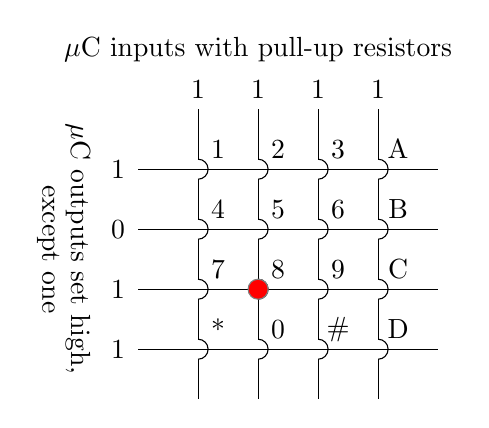
\begin{tikzpicture}[x=.1in, y=.1in]
            \draw (7,10) node {1} +(3,0) node {2} +(6,0) node {3} +(9,0) node {A}
            +(0,-3) node {4} +(3,-3) node {5} +(6,-3) node {6} +(9,-3) node {B}
            +(0,-6) node {7} +(3,-6) node {8} +(6,-6) node {9} +(9,-6) node {C}
            +(0,-9) node {*} +(3,-9) node {0} +(6,-9) node {\#} +(9,-9) node {D};
            \draw (0,5) node {\rotatebox{-90}{$\mu$C outputs set high,}};
            \draw (-1.5,5) node {\rotatebox{-90}{except one}};
            \draw (0,9) +(2,0) node {1} ++(3,0) -- ++(15,0);
            \draw (0,6) +(2,0) node {0} ++(3,0) -- ++(15,0);
            \draw (0,3) +(2,0) node {1} ++(3,0) -- ++(15,0);
            \draw (0,0) +(2,0) node {1} ++(3,0) -- ++(15,0);
            \draw (9,15) node {$\mu$C inputs with pull-up resistors};
            \draw (6,15) +(0,-2) node {1} ++(0,-3) -- ++(0,-2.5) ++(0,-1) -- ++(0,-2) ++(0,-1) -- ++(0,-2) ++(0,-1) -- ++(0,-2) ++(0,-1) -- ++(0,-2);
            \draw (6,9.5) arc [start angle=90, end angle=-90, radius=.5] ++(0,-2) arc [start angle=90, end angle=-90, radius=.5] ++(0,-2) arc [start angle=90, end angle=-90, radius=.5] ++(0,-2) arc [start angle=90, end angle=-90, radius=.5];
            \draw (9,15) +(0,-2) node {1} ++(0,-3) -- ++(0,-2.5) ++(0,-1) -- ++(0,-2) ++(0,-1) -- ++(0,-2) ++(0,-1) -- ++(0,-2) ++(0,-1) -- ++(0,-2);
            \draw (9,9.5) arc [start angle=90, end angle=-90, radius=.5] ++(0,-2) arc [start angle=90, end angle=-90, radius=.5] ++(0,-2) arc [start angle=90, end angle=-90, radius=.5] ++(0,-2) arc [start angle=90, end angle=-90, radius=.5];
            \draw (12,15) +(0,-2) node {1} ++(0,-3) -- ++(0,-2.5) ++(0,-1) -- ++(0,-2) ++(0,-1) -- ++(0,-2) ++(0,-1) -- ++(0,-2) ++(0,-1) -- ++(0,-2);
            \draw (12,9.5) arc [start angle=90, end angle=-90, radius=.5] ++(0,-2) arc [start angle=90, end angle=-90, radius=.5] ++(0,-2) arc [start angle=90, end angle=-90, radius=.5] ++(0,-2) arc [start angle=90, end angle=-90, radius=.5];
            \draw (15,15) +(0,-2) node {1} ++(0,-3) -- ++(0,-2.5) ++(0,-1) -- ++(0,-2) ++(0,-1) -- ++(0,-2) ++(0,-1) -- ++(0,-2) ++(0,-1) -- ++(0,-2);
            \draw (15,9.5) arc [start angle=90, end angle=-90, radius=.5] ++(0,-2) arc [start angle=90, end angle=-90, radius=.5] ++(0,-2) arc [start angle=90, end angle=-90, radius=.5] ++(0,-2) arc [start angle=90, end angle=-90, radius=.5];
            \draw[gray, fill=red] (9,3) circle (.5);
        \end{tikzpicture}
    }
    \hfill
    \subfloat[Examining a row that does have a pressed key.]{
        \centering
        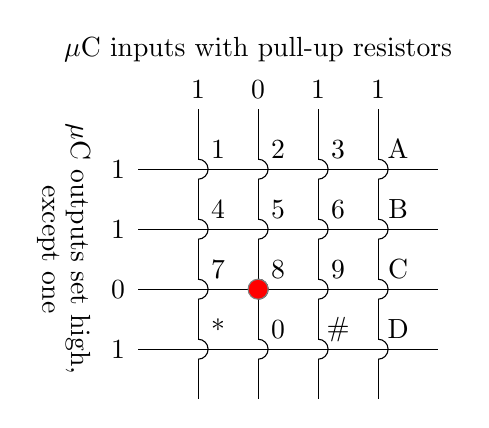
\begin{tikzpicture}[x=.1in, y=.1in]
            \draw (7,10) node {1} +(3,0) node {2} +(6,0) node {3} +(9,0) node {A}
            +(0,-3) node {4} +(3,-3) node {5} +(6,-3) node {6} +(9,-3) node {B}
            +(0,-6) node {7} +(3,-6) node {8} +(6,-6) node {9} +(9,-6) node {C}
            +(0,-9) node {*} +(3,-9) node {0} +(6,-9) node {\#} +(9,-9) node {D};
            \draw (0,5) node {\rotatebox{-90}{$\mu$C outputs set high,}};
            \draw (-1.5,5) node {\rotatebox{-90}{except one}};
            \draw (0,9) +(2,0) node {1} ++(3,0) -- ++(15,0);
            \draw (0,6) +(2,0) node {1} ++(3,0) -- ++(15,0);
            \draw (0,3) +(2,0) node {0} ++(3,0) -- ++(15,0);
            \draw (0,0) +(2,0) node {1} ++(3,0) -- ++(15,0);
            \draw (9,15) node {$\mu$C inputs with pull-up resistors};
            \draw (6,15) +(0,-2) node {1} ++(0,-3) -- ++(0,-2.5) ++(0,-1) -- ++(0,-2) ++(0,-1) -- ++(0,-2) ++(0,-1) -- ++(0,-2) ++(0,-1) -- ++(0,-2);
            \draw (6,9.5) arc [start angle=90, end angle=-90, radius=.5] ++(0,-2) arc [start angle=90, end angle=-90, radius=.5] ++(0,-2) arc [start angle=90, end angle=-90, radius=.5] ++(0,-2) arc [start angle=90, end angle=-90, radius=.5];
            \draw (9,15) +(0,-2) node {0} ++(0,-3) -- ++(0,-2.5) ++(0,-1) -- ++(0,-2) ++(0,-1) -- ++(0,-2) ++(0,-1) -- ++(0,-2) ++(0,-1) -- ++(0,-2);
            \draw (9,9.5) arc [start angle=90, end angle=-90, radius=.5] ++(0,-2) arc [start angle=90, end angle=-90, radius=.5] ++(0,-2) arc [start angle=90, end angle=-90, radius=.5] ++(0,-2) arc [start angle=90, end angle=-90, radius=.5];
            \draw (12,15) +(0,-2) node {1} ++(0,-3) -- ++(0,-2.5) ++(0,-1) -- ++(0,-2) ++(0,-1) -- ++(0,-2) ++(0,-1) -- ++(0,-2) ++(0,-1) -- ++(0,-2);
            \draw (12,9.5) arc [start angle=90, end angle=-90, radius=.5] ++(0,-2) arc [start angle=90, end angle=-90, radius=.5] ++(0,-2) arc [start angle=90, end angle=-90, radius=.5] ++(0,-2) arc [start angle=90, end angle=-90, radius=.5];
            \draw (15,15) +(0,-2) node {1} ++(0,-3) -- ++(0,-2.5) ++(0,-1) -- ++(0,-2) ++(0,-1) -- ++(0,-2) ++(0,-1) -- ++(0,-2) ++(0,-1) -- ++(0,-2);
            \draw (15,9.5) arc [start angle=90, end angle=-90, radius=.5] ++(0,-2) arc [start angle=90, end angle=-90, radius=.5] ++(0,-2) arc [start angle=90, end angle=-90, radius=.5] ++(0,-2) arc [start angle=90, end angle=-90, radius=.5];
            \draw[gray, fill=red] (9,3) circle (.5);
        \end{tikzpicture}
    }
    \hspace{.5in}
    \caption{Scanning a matrix keypad. The red dot indicates which key is being pressed.} \label{fig:scanning-keypad}
\end{figure}

After the code has determined which row and column the pressed key is on, it can return a value or assign a value to a variable accordingly.
This might be a \lstinline{char} corresponding to the character on the key's face, as is the case for \function{cowpi_get_keypress} (Section~\ref{subsec:ScannedInputs}).
Or this might be an \lstinline{int} corresponding to the value of the numeral on the key's face.
Or this might even be some value unrelated to whatever is printed on the key's face.

\subsubsection{Scanning the Keypad}

There are a few options for obtaining the value corresponding to a key that is pressed on the keypad.
The most efficient for a simple application is to use a lookup table.
For example, if you need to return a character that corresponds to the face value of the key that was pressed, then the lookup table would be:
\[
    keys \gets
    \left(\begin{array}{cccc}
              '1' & '2' & '3' & 'A' \\
              '4' & '5' & '6' & 'B' \\
              '7' & '8' & '9' & 'C' \\
              '*' & '0' & '\#' & 'D'
    \end{array}\right)
\]

If the keypad is wired to the \mcuboard\ such that four contiguous output pins are connected to the rows and four contiguous input pins are connected to the columns (as is the case for the Cow Pi), then this pseudocode will scan the keypad and determine which key, if any, is pressed:
Note that this pseudocode will report at most one key pressed;
it would have to be modified to report multiple keys pressed.
(This is not a limitation for mark~1 Cow Pis, as their keypads are wired without protection against shorting power to ground when two keys are pressed simultaneously.)

\begin{lstlisting}[language=pascal,basicstyle=\rmfamily\footnotesize,literate={:=}{{$\gets$}}1 {<=}{{$\leq$}}1 {>=}{{$\geq$}}1 {<>}{{$\neq$}}1 {->}{{$\succ$}}1]
for each row:
    row_bit_vector := 0b1111    (* set all rows to 1 *)
    row_bit_vector(row) := 0    (* except the row we're currently examining *)
    wait at least one microcontroller clock cycle
    for each column:
        if (column_bit_vector(column) = 0):
            key_pressed := keys(row,column)
row_bit_vector := 0b0000        (* set all rows to 0 to detect the next keypress *)
\end{lstlisting}

The delay shown in line 4 is sometimes, but not always necessary.
There is a slight delay between setting a pin's output value and being able to detect the change by reading a different pin's input value.
Some realizations of the pseudocode attempt to read the change before it can be read reliably;
this usually manifests as one of the keypad's columns not being readable.
The fix is to introduce a delay of at least one clock cycle (strictly speaking, one clock cycle is more than enough, but a shorter delay is not possible).
This could be managed by introducing a delay based on the microcontroller's clock cycle, using the AVR-libc \function{_NOP()} or \function{_delay_loop_1()} functions,\cite{avrNOP}\cite{avrDelayBasic} to be able to introduce a delay of exactly one or three clock cycles (\function{_NOP()} or \function{_delay_loop_1(1)}, respectively),
or this could be managed by introducing a 1$\mu$s delay using the Arduino core library's \function{delayMicroseconds()} function,\cite{arduinoDelay} which is portable across all devices using the Arduino toolchain.

\subsection{Display Module}

The display module used in the \hardwareversion~Cow Pi is a \displaymoduledescription.
A full description of its control signals can be found in the HD44780U datasheet;\cite{lcd1602}
however, the CowPi library's functions handles these control signals -- see Section~\ref{subsec:DisplayModules}.
If a function to send a halfbyte to the display module is registered, either the CowPi library's default implementation or your own (Section~\ref{subsubsec:send_halfbyte}), then you do not need to manage the control signals.

Displaying useful information on the display module does require some awareness of the dipslay module's characteristics.
As previously stated, the display module can display up to 32 characters, 16 characters on each of two rows.
When sending these characters using the library's \hyperlink{function:cowpi_lcd1602_place_character}{\function{cowpi_lcd1602_place_character()}} or \hyperlink{function:cowpi_lcd1602_send_character}{\function{cowpi_lcd1602_send_character()}} functions, you typically can use standard ASCII characters.
Specifically, if the \lstinline{character} argument is in the range 0x20--0x7D, then the corresponding ASCII character will be displayed.
For the characters displayed when the argument is 0x7E, 0x7F, or in the range 0xA1--0xFF, see Table~4 of the HD44780U datasheet.\cite{lcd1602}
Up to eight custom characters can also be created; see the \hyperlink{function:cowpi_lcd1602_create_character}{\function{cowpi_lcd1602_create_character()}} function and the \textit{lcd1602\_custom\_characters} example program described in Section~\ref{subsec:CustomCharacters}.

While there are 16 characters displayed per row, the display module has memory addresses for 40 characters per row.
The base address of the top row is 0x00, and the base address of the bottom row is 0x40.
Initially, the characters at addresses 0x00--0x0F and 0x40--0x4F are displayed, as shown in Figure~\ref{fig:initial-display}.

\begin{figure}[t]
    \centering
    \tiny
    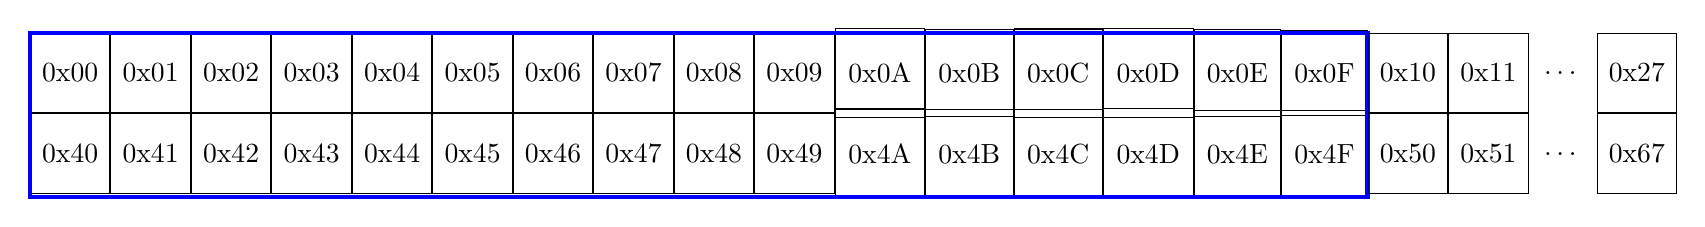
\begin{tikzpicture}[x=.1in, y=.1in, square/.style={regular polygon,regular polygon sides=4,inner sep=0,minimum size=1.2cm}]
        \node at (0,0) [square,draw,anchor=west] (0x00) {0x00};
        \node at (0x00.east) [square,draw,anchor=west] (0x01) {0x01};
        \node at (0x01.east) [square,draw,anchor=west] (0x02) {0x02};
        \node at (0x02.east) [square,draw,anchor=west] (0x03) {0x03};
        \node at (0x03.east) [square,draw,anchor=west] (0x04) {0x04};
        \node at (0x04.east) [square,draw,anchor=west] (0x05) {0x05};
        \node at (0x05.east) [square,draw,anchor=west] (0x06) {0x06};
        \node at (0x06.east) [square,draw,anchor=west] (0x07) {0x07};
        \node at (0x07.east) [square,draw,anchor=west] (0x08) {0x08};
        \node at (0x08.east) [square,draw,anchor=west] (0x09) {0x09};
        \node at (0x09.east) [square,draw,anchor=west] (0x0A) {0x0A};
        \node at (0x0A.east) [square,draw,anchor=west] (0x0B) {0x0B};
        \node at (0x0B.east) [square,draw,anchor=west] (0x0C) {0x0C};
        \node at (0x0C.east) [square,draw,anchor=west] (0x0D) {0x0D};
        \node at (0x0D.east) [square,draw,anchor=west] (0x0E) {0x0E};
        \node at (0x0E.east) [square,draw,anchor=west] (0x0F) {0x0F};
        \node at (0x00.south) [square,draw,anchor=north] (0x40) {0x40};
        \node at (0x40.east) [square,draw,anchor=west] (0x41) {0x41};
        \node at (0x41.east) [square,draw,anchor=west] (0x42) {0x42};
        \node at (0x42.east) [square,draw,anchor=west] (0x43) {0x43};
        \node at (0x43.east) [square,draw,anchor=west] (0x44) {0x44};
        \node at (0x44.east) [square,draw,anchor=west] (0x45) {0x45};
        \node at (0x45.east) [square,draw,anchor=west] (0x46) {0x46};
        \node at (0x46.east) [square,draw,anchor=west] (0x47) {0x47};
        \node at (0x47.east) [square,draw,anchor=west] (0x48) {0x48};
        \node at (0x48.east) [square,draw,anchor=west] (0x49) {0x49};
        \node at (0x49.east) [square,draw,anchor=west] (0x4A) {0x4A};
        \node at (0x4A.east) [square,draw,anchor=west] (0x4B) {0x4B};
        \node at (0x4B.east) [square,draw,anchor=west] (0x4C) {0x4C};
        \node at (0x4C.east) [square,draw,anchor=west] (0x4D) {0x4D};
        \node at (0x4D.east) [square,draw,anchor=west] (0x4E) {0x4E};
        \node at (0x4E.east) [square,draw,anchor=west] (0x4F) {0x4F};
        \draw[blue,ultra thick] (0x00.north west) rectangle (0x4F.south east);
        \node at (0x0F.east) [square,draw,anchor=west] (0x10) {0x10};
        \node at (0x4F.east) [square,draw,anchor=west] (0x50) {0x50};
        \node at (0x10.east) [square,draw,anchor=west] (0x11) {0x11};
        \node at (0x50.east) [square,draw,anchor=west] (0x51) {0x51};
        \node at (0x11.east) [white,square,draw,anchor=west] (dots0) {$\dots$};
        \node at (0x51.east) [white,square,draw,anchor=west] (dots1) {$\dots$};
        \draw (dots0.center) node {$\dots$};
        \draw (dots1.center) node {$\dots$};
        \node at (dots0.east) [square,draw,anchor=west] (0x27) {0x27};
        \node at (dots1.east) [square,draw,anchor=west] (0x67) {0x67};
    \end{tikzpicture}
    \caption{Initially, the characters at addresses 0x00--0x0F and 0x40--0x4F are displayed. The black squares are character memory locations; the blue rectangle shows which characters are displayed.} \label{fig:initial-display}
\end{figure}

The displayed addresses can shift to the left or to the right.
Normally the display will not shift when a character is displayed; however, the display can be configured to shift with each new character added.
This is achieved by changing the entry mode with the \hyperlink{function:cowpi_lcd1602_send_command}{\function{cowpi_lcd1602_send_command()}} function.
Alternatively, the display can be explicitly shifted, regardless of the entry mode. If the \hyperlink{function:cowpi_lcd1602_send_command}{\function{cowpi_lcd1602_send_command()}} function is used so send the \lstinline{LCDSHIFT_DISPLAYLEFT} or the \lstinline{LCD_DISPLAY_RIGHT} command, then the display will shift to the left or to the right accordingly.

For example, if the display is shifted to the left from its initial configuration, then the characters at addresses 0x01--0x10 and 0x41--0x50 are displayed, as shown in Figure~\ref{fig:shiftleft-display}.

\begin{figure}[t]
    \centering
    \tiny
    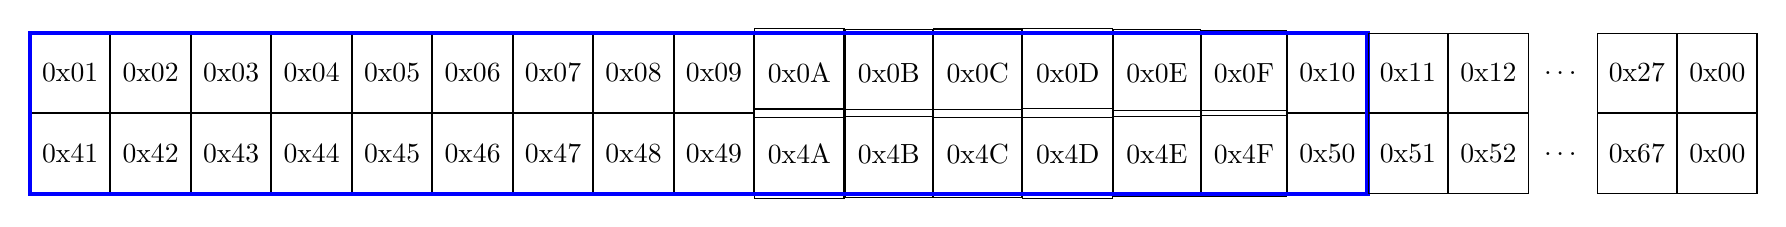
\begin{tikzpicture}[x=.1in, y=.1in, square/.style={regular polygon,regular polygon sides=4,inner sep=0,minimum size=1.2cm}]
        \node at (0,0) [square,draw,anchor=west] (0x01) {0x01};
        \node at (0x01.east) [square,draw,anchor=west] (0x02) {0x02};
        \node at (0x02.east) [square,draw,anchor=west] (0x03) {0x03};
        \node at (0x03.east) [square,draw,anchor=west] (0x04) {0x04};
        \node at (0x04.east) [square,draw,anchor=west] (0x05) {0x05};
        \node at (0x05.east) [square,draw,anchor=west] (0x06) {0x06};
        \node at (0x06.east) [square,draw,anchor=west] (0x07) {0x07};
        \node at (0x07.east) [square,draw,anchor=west] (0x08) {0x08};
        \node at (0x08.east) [square,draw,anchor=west] (0x09) {0x09};
        \node at (0x09.east) [square,draw,anchor=west] (0x0A) {0x0A};
        \node at (0x0A.east) [square,draw,anchor=west] (0x0B) {0x0B};
        \node at (0x0B.east) [square,draw,anchor=west] (0x0C) {0x0C};
        \node at (0x0C.east) [square,draw,anchor=west] (0x0D) {0x0D};
        \node at (0x0D.east) [square,draw,anchor=west] (0x0E) {0x0E};
        \node at (0x0E.east) [square,draw,anchor=west] (0x0F) {0x0F};
        \node at (0x01.south) [square,draw,anchor=north] (0x41) {0x41};
        \node at (0x41.east) [square,draw,anchor=west] (0x42) {0x42};
        \node at (0x42.east) [square,draw,anchor=west] (0x43) {0x43};
        \node at (0x43.east) [square,draw,anchor=west] (0x44) {0x44};
        \node at (0x44.east) [square,draw,anchor=west] (0x45) {0x45};
        \node at (0x45.east) [square,draw,anchor=west] (0x46) {0x46};
        \node at (0x46.east) [square,draw,anchor=west] (0x47) {0x47};
        \node at (0x47.east) [square,draw,anchor=west] (0x48) {0x48};
        \node at (0x48.east) [square,draw,anchor=west] (0x49) {0x49};
        \node at (0x49.east) [square,draw,anchor=west] (0x4A) {0x4A};
        \node at (0x4A.east) [square,draw,anchor=west] (0x4B) {0x4B};
        \node at (0x4B.east) [square,draw,anchor=west] (0x4C) {0x4C};
        \node at (0x4C.east) [square,draw,anchor=west] (0x4D) {0x4D};
        \node at (0x4D.east) [square,draw,anchor=west] (0x4E) {0x4E};
        \node at (0x4E.east) [square,draw,anchor=west] (0x4F) {0x4F};
        \node at (0x0F.east) [square,draw,anchor=west] (0x10) {0x10};
        \node at (0x4F.east) [square,draw,anchor=west] (0x50) {0x50};
        \draw[blue,ultra thick] (0x01.north west) rectangle (0x50.south east);
        \node at (0x10.east) [square,draw,anchor=west] (0x11) {0x11};
        \node at (0x50.east) [square,draw,anchor=west] (0x51) {0x51};
        \node at (0x11.east) [square,draw,anchor=west] (0x12) {0x12};
        \node at (0x51.east) [square,draw,anchor=west] (0x52) {0x52};
        \node at (0x12.east) [white,square,draw,anchor=west] (dots0) {$\dots$};
        \node at (0x52.east) [white,square,draw,anchor=west] (dots1) {$\dots$};
        \draw (dots0.center) node {$\dots$};
        \draw (dots1.center) node {$\dots$};
        \node at (dots0.east) [square,draw,anchor=west] (0x27) {0x27};
        \node at (dots1.east) [square,draw,anchor=west] (0x67) {0x67};
        \node at (0x27.east) [square,draw,anchor=west] (0x00) {0x00};
        \node at (0x67.east) [square,draw,anchor=west] (0x00) {0x00};
    \end{tikzpicture}
    \caption{After shifting the display to the left, the characters at addresses 0x01--0x10 and 0x41--0x50 are displayed. The black squares are character memory locations; the blue rectangle shows which characters are displayed.} \label{fig:shiftleft-display}
\end{figure}

If, when shifting, one ``end'' of the rows or the other is passed, then the display ``wraps'' around, displaying some characters at both ends of the rows' addresses.
For example, if the display is shifted to the right from its initial configuration, then the characters at addresses 0x27, 0x00--0x0E and 0x67, 0x40--0x4E are displayed, as shown in Figure~\ref{fig:shiftright-display}.

\begin{figure}[h]
    \centering
    \tiny
    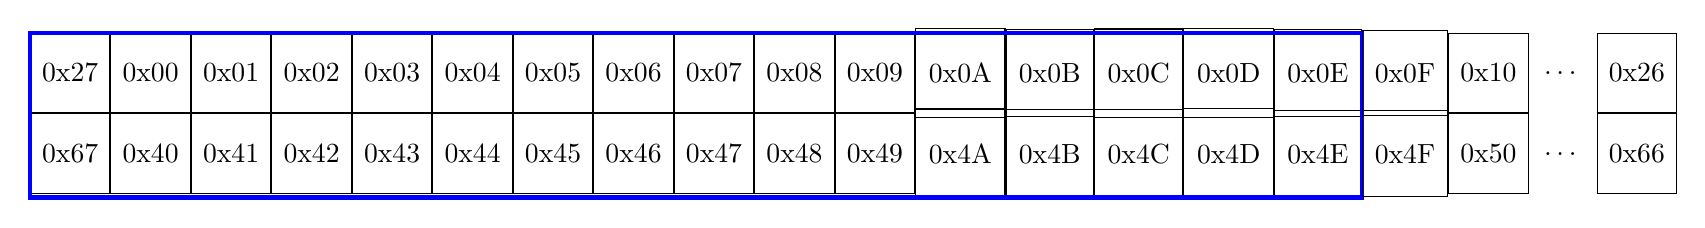
\begin{tikzpicture}[x=.1in, y=.1in, square/.style={regular polygon,regular polygon sides=4,inner sep=0,minimum size=1.2cm}]
        \node at (0,0) [square,draw,anchor=west] (0x27) {0x27};
        \node at (0x27.east) [square,draw,anchor=west] (0x00) {0x00};
        \node at (0x00.east) [square,draw,anchor=west] (0x01) {0x01};
        \node at (0x01.east) [square,draw,anchor=west] (0x02) {0x02};
        \node at (0x02.east) [square,draw,anchor=west] (0x03) {0x03};
        \node at (0x03.east) [square,draw,anchor=west] (0x04) {0x04};
        \node at (0x04.east) [square,draw,anchor=west] (0x05) {0x05};
        \node at (0x05.east) [square,draw,anchor=west] (0x06) {0x06};
        \node at (0x06.east) [square,draw,anchor=west] (0x07) {0x07};
        \node at (0x07.east) [square,draw,anchor=west] (0x08) {0x08};
        \node at (0x08.east) [square,draw,anchor=west] (0x09) {0x09};
        \node at (0x09.east) [square,draw,anchor=west] (0x0A) {0x0A};
        \node at (0x0A.east) [square,draw,anchor=west] (0x0B) {0x0B};
        \node at (0x0B.east) [square,draw,anchor=west] (0x0C) {0x0C};
        \node at (0x0C.east) [square,draw,anchor=west] (0x0D) {0x0D};
        \node at (0x0D.east) [square,draw,anchor=west] (0x0E) {0x0E};
        \node at (0x27.south) [square,draw,anchor=north] (0x67) {0x67};
        \node at (0x67.east) [square,draw,anchor=west] (0x40) {0x40};
        \node at (0x40.east) [square,draw,anchor=west] (0x41) {0x41};
        \node at (0x41.east) [square,draw,anchor=west] (0x42) {0x42};
        \node at (0x42.east) [square,draw,anchor=west] (0x43) {0x43};
        \node at (0x43.east) [square,draw,anchor=west] (0x44) {0x44};
        \node at (0x44.east) [square,draw,anchor=west] (0x45) {0x45};
        \node at (0x45.east) [square,draw,anchor=west] (0x46) {0x46};
        \node at (0x46.east) [square,draw,anchor=west] (0x47) {0x47};
        \node at (0x47.east) [square,draw,anchor=west] (0x48) {0x48};
        \node at (0x48.east) [square,draw,anchor=west] (0x49) {0x49};
        \node at (0x49.east) [square,draw,anchor=west] (0x4A) {0x4A};
        \node at (0x4A.east) [square,draw,anchor=west] (0x4B) {0x4B};
        \node at (0x4B.east) [square,draw,anchor=west] (0x4C) {0x4C};
        \node at (0x4C.east) [square,draw,anchor=west] (0x4D) {0x4D};
        \node at (0x4D.east) [square,draw,anchor=west] (0x4E) {0x4E};
        \draw[blue,ultra thick] (0x27.north west) rectangle (0x4E.south east);
        \node at (0x0E.east) [square,draw,anchor=west] (0x0F) {0x0F};
        \node at (0x4E.east) [square,draw,anchor=west] (0x4F) {0x4F};
        \node at (0x0F.east) [square,draw,anchor=west] (0x10) {0x10};
        \node at (0x4F.east) [square,draw,anchor=west] (0x50) {0x50};
        \node at (0x10.east) [white,square,draw,anchor=west] (dots0) {$\dots$};
        \node at (0x50.east) [white,square,draw,anchor=west] (dots1) {$\dots$};
        \draw (dots0.center) node {$\dots$};
        \draw (dots1.center) node {$\dots$};
        \node at (dots0.east) [square,draw,anchor=west] (0x26) {0x26};
        \node at (dots1.east) [square,draw,anchor=west] (0x66) {0x66};
    \end{tikzpicture}
    \caption{When shifting, the display ``wraps'' around the rows' addresses. The black squares are character memory locations; the blue rectangle shows which characters are displayed.} \label{fig:shiftright-display}
\end{figure}




    \section{Library Overview} %! suppress = NonMatchingIf
This section describes the v\softwareversion\ CowPi library's functions relevant to the Cow Pi \cowpiversion\ development board.
More complete documentation can be obtained by processing the library's source code with Doxygen.
% I, too, wish that I could simply use Doxygen's output here

\subsection{Configuring / Initializing the Board}

    Functions used to configure the Cow Pi hardware and library at the start of a program.

    \begin{itemize}
        \functionitem{void}{cowpi_setup}{unsigned int configuration} \\ \\
            Configures the microcontroller's pins for the expected hardware setup, and configures the library to work with the specified display module and communication protocol.
            \begin{description}
                \item[parameters] \
                    \begin{description}
                        \item[configuration] bitwise disjunction of named constants, specifying the display module and protocol
                            \begin{itemize}
                                \item For the Cow Pi \cowpiversion, the typical argument will be
                                    \ifdefstring{\cowpiversion}{mk1c}{\texttt{MAX7219|SPI}}{}
                                    \ifdefstring{\cowpiversion}{mk1d}{\texttt{LCD1602|I2C}}{}
                                    \ifdefstring{\cowpiversion}{mk3a}{either \texttt{LCD1602|SPI} or \texttt{LCD1602|I2C}, depending on how the development board is configured}{}
                            \end{itemize}
                    \end{description}
                \item[returns] n/a
                \item[notes] \
                    \begin{itemize}
                        \item If the I$^2$C protocol is used, then \function{cowpi_set_display_i2c_address()} must be called \textit{before} \function{cowpi_setup()}
                        \ifboolexpe{bool{lcd1602}}{\item If a non-\lstinline{COWPI_DEFAULT} display dialect is used, then \function{cowpi_set_display_dialect()} must be called before \function{cowpi_setup()}}{}
                        \ifdefstring{\microcontroller}{ATmega328P}{\item If \function{printf()} and/or \function{scanf()} will be used, then we recommend that \function{cowpi_stdio_setup()} be called before \function{cowpi_setup()}; however, this is not required}{}
                    \end{itemize}
            \end{description}

        \ifboolexpe{bool{i2c}}{\functionitem{void}{cowpi_set_display_i2c_address}{uint8_t peripheral_address} \\ \\
            Sets the I$^2$C address for an I$^2$C-driven display module. \\ \\
            Because the I$^2$C protocol uses addresses to select the peripheral that the microcontroller is communicating with, the display module's address needs to be set.
            If the SPI protocol is being used, then there is no need to call this function. \\ \\
            The common PCF8574-based interfaces used with LCD1602 display modules typically have an address of 0x27, and we have encountered some interfaces with an address of 0x3F, but these addresses can readily be changed.
            \begin{description}
                \item[parameters] \
                \begin{description}
                    \item[peripheral\_address]
                \end{description}
                \item[returns] n/a
                \item[notes] \
                \begin{itemize}
                    \item If this function is called, it must be called before \function{cowpi_setup()} so that the display module can be properly configured.
                \end{itemize}
            \end{description}
        }{}

        \ifboolexpe{bool{lcd1602}}{\functionitem{void}{cowpi_set_display_dialect}{uint8_t dialect} \\ \\
            Sets the ``dialect,'' or the mapping of protocol bits to display module bits. \\ \\
            Some display modules (e.g., MAX7219-based modules) have only one possible mapping, and calling this function has no effect for those modules.
            For other display modules, the \lstinline{COWPI_DEFAULT} dialect is the default;
            this function does not need to be called if the \lstinline{COWPI_DEFAULT} dialect will be used.
            \begin{description}
                \item[parameters] \
                \begin{description}
                    \item[dialect] a named constant specifying which mapping of protocol bits to display module bits shall be used
                \end{description}
                \item[returns] n/a
                \item[notes] \
                \begin{itemize}
                    \item If this function is called, it must be called before \function{cowpi_setup()} so that the display module can be properly configured.
                \end{itemize}
            \end{description}
        }{}

        \ifdefstring{\microcontroller}{ATmega328P}{\functionitem{void}{cowpi_stdio_setup}{unsigned long baud} \\ \\
            Configures the CowPi library to use \textit{stdio.h} functions. \\ \\
            Configures \function{printf()} to write to, and \function{scanf()} to read from, the serial interface between the microcontroller and the host computer.
            Calls to \function{printf()} and \function{scanf()} that occur before the call to \function{cowpi_stdio_setup()} will have no effect.
            \begin{description}
                \item[parameters] \
                \begin{description}
                    \item[baud] the USART signal rate
                \end{description}
                \item[returns] n/a
                \item[notes] \
                \begin{itemize}
                    \item By default, \function{printf()} will not format floating point numbers%;
                        %to override this behavior, add \texttt{\#define printf} to the start of your program <-- for mbed -- also, maybe #undefine? -- but for avr-libc, requires linking to a library (https://www.nongnu.org/avr-libc/user-manual/group__avr__stdio.html)
                \end{itemize}
            \end{description}
        }{}

    \end{itemize}


\subsection{Simple Inputs}\label{subsec:SimpleInputs}

    Buttons and switches that can be read directly from pins.

    \begin{itemize}
        \functionitem{bool}{cowpi_left_button_is_pressed}{void} \\ \\
        Reports whether the left button is pressed. \\ \\
            There is no debouncing.
            This is a portable implementation, not a memory-mapped implementation. \\ \\
            Assumes the left button is in Arduino pin D8.
            A pressed button grounds a pulled-high input.
            \begin{description}
                \item[parameters] n/a
                \item[returns] \lstinline{true} if the button is pressed, \lstinline{false} otherwise
                %\item[notes]
            \end{description}

        \functionitem{bool}{cowpi_right_button_is_pressed}{void} \\ \\
        Reports whether the right button is pressed. \\ \\
        There is no debouncing.
        This is a portable implementation, not a memory-mapped implementation. \\ \\
        Assumes the left button is in Arduino pin D9.
        A pressed button grounds a pulled-high input.
        \begin{description}
            \item[parameters] n/a
            \item[returns] \lstinline{true} if the button is pressed, \lstinline{false} otherwise
            %\item[notes]
        \end{description}

        \functionitem{bool}{cowpi_left_switch_is_in_left_position}{void} \\ \\
        Reports whether the left switch is in the left position. \\ \\
            There is no debouncing.
            This is a portable implementation, not a memory-mapped implementation. \\ \\
            Assumes the left switch is in Arduino pin A4 (D18) if SPI (but not I$^2$C) is in use or if no protocol is in use;
            assumes the switch is in pin D11 if I$^2$C (but not SPI) is in use.
            If both protocols are in use, then this function will always return \lstinline{false}.
            A switch in the left position grounds a pulled-high input.
            \begin{description}
                \item[parameters] n/a
                \item[returns] \lstinline{true} if the switch is in the left position, \lstinline{false} otherwise
                %\item[notes]
            \end{description}

        \functionitem{bool}{cowpi_left_switch_is_in_right_position}{void} \\ \\
        Reports whether the left switch is in the right position. \\ \\
        There is no debouncing.
        This is a portable implementation, not a memory-mapped implementation. \\ \\
        Assumes the left switch is in Arduino pin A4 (D18) if SPI (but not I$^2$C) is in use or if no protocol is in use;
        assumes the switch is in pin D11 if I$^2$C (but not SPI) is in use.
        If both protocols are in use, then this function will always return \lstinline{false}.
        A switch in the right position floats, allowing a pulled-high input to remain high.
        \begin{description}
            \item[parameters] n/a
            \item[returns] \lstinline{true} if the switch is in the right position, \lstinline{false} otherwise
            %\item[notes]
        \end{description}

        \functionitem{bool}{cowpi_right_switch_is_in_left_position}{void} \\ \\
        Reports whether the right switch is in the left position. \\ \\
        There is no debouncing.
        This is a portable implementation, not a memory-mapped implementation. \\ \\
        Assumes the right switch is in Arduino pin A5 (D19) if SPI (but not I$^2$C) is in use or if no protocol is in use;
        assumes the switch is in pin D10 if I$^2$C (but not SPI) is in use.
        If both protocols are in use, then this function will always return \lstinline{false}.
        A switch in the left position grounds a pulled-high input.
        \begin{description}
            \item[parameters] n/a
            \item[returns] \lstinline{true} if the switch is in the left position, \lstinline{false} otherwise
            %\item[notes]
        \end{description}

        \functionitem{bool}{cowpi_right_switch_is_in_right_position}{void} \\ \\
        Reports whether the right switch is in the right position. \\ \\
        There is no debouncing.
        This is a portable implementation, not a memory-mapped implementation. \\ \\
        Assumes the right switch is in Arduino pin A5 (D19) if SPI (but not I$^2$C) is in use or if no protocol is in use;
        assumes the switch is in pin D10 if I$^2$C (but not SPI) is in use.
        If both protocols are in use, then this function will always return \lstinline{false}.
        A switch in the right position floats, allowing a pulled-high input to remain high.
        \begin{description}
            \item[parameters] n/a
            \item[returns] \lstinline{true} if the switch is in the right position, \lstinline{false} otherwise
            %\item[notes]
        \end{description}

    \end{itemize}


\subsection{Simple Outputs}\label{subsec:SimpleOutputs}

    LEDs that can be written directly through pins.

    \begin{itemize}
        \functionitem{void}{cowpi_illuminate_left_led}{void} \\ \\
            Illuminates the left LED, aka the built-in LED, aka the internal LED\@.
            This is a portable implementation, not a memory-mapped implementation. \\ \\
            Assumes the left LED is on Arduino pin D13. \\ \\
            The Arduino semantics are that an LED illuminates when the pin is placed high.
            \begin{description}
                \item[parameters] n/a
                \item[returns] n/a
                %\item[notes]
            \end{description}

        \functionitem{void}{cowpi_deluminate_left_led}{void} \\ \\
            Deluminates the left LED, aka the built-in LED, aka the internal LED\@.
            This is a portable implementation, not a memory-mapped implementation. \\ \\
            Assumes the left LED is on Arduino pin D13. \\ \\
            The Arduino semantics are that an LED deluminates when the pin is placed low.
            \begin{description}
                \item[parameters] n/a
                \item[returns] n/a
                %\item[notes]
            \end{description}

        \functionitem{void}{cowpi_illuminate_right_led}{void} \\ \\
            Illuminates the right LED, aka the external LED\@.
            This is a portable implementation, not a memory-mapped implementation. \\ \\
            Assumes the right LED is on Arduino pin D12. \\ \\
            An LED illuminates when the pin is placed high, to match the semantics of Arduino's built-in LED\@.
            \begin{description}
                \item[parameters] n/a
                \item[returns] n/a
                %\item[notes]
            \end{description}

        \functionitem{void}{cowpi_deluminate_right_led}{void} \\ \\
            Deluminates the right LED, aka the external LED\@.
            This is a portable implementation, not a memory-mapped implementation. \\ \\
            Assumes the right LED is on Arduino pin D12. \\ \\
            An LED deluminates when the pin is placed low, to match the semantics of Arduino's built-in LED\@.
            \begin{description}
                \item[parameters] n/a
                \item[returns] n/a
                %\item[notes]
            \end{description}

    \end{itemize}


    \subsection{Scanned Inputs}\label{subsec:ScannedInputs}

        Keypad that is scanned through a combination of writing to pins and reading from other pins.

        \begin{itemize}
            \functionitem{char}{cowpi_get_keypress}{void} \\ \\
            Scans the keypad to determine which, if any, key was pressed. \\ \\
            There is no debouncing.
            This is a portable implementation, not a memory-mapped implementation.
            Returns the ASCII representation of the character depicted on whichever key was pressed (0-9, A-D, *, \#). \\ \\
            Assumes a common 4x4 matrix keypad with the rows in Arduino pins D4-D7 and the columns in Arduino pins A0-A3 (D14-D17).
            A pressed key grounds a pulled-high input.
            \begin{description}
                \item[parameters] n/a
                \item[returns] ASCII character corresponding to the key that is pressed, or \texttt{NUL} if no key is pressed
                %\item[notes]
            \end{description}

        \end{itemize}


    \subsection{Display Modules}\label{subsec:DisplayModules}

    Functions for display modules.

    \begin{itemize}
        \ifboolexpe{bool{max7219digits} or bool{max7219matrix}}{
            \functionitem{void}{cowpi_max7219_send}{uint8_t address, uint8_t data} \\ \\
                Sends a byte of data to be placed in the specified MAX7219 register. \\ \\
                The firmware program should only need to send data to addresses 1--8, the digit registers.
                Most other registers are handled by specific \function{cowpi_max7219} functions. \\ \\
                This is a portable software-only implementation;
                it does not use SPI hardware, nor does it use memory-mapped I/O of any form.
                Re-implementing this function (using a different function name) to use SPI hardware is a possible part of a memory-mapped I/O lab assignment.
                \begin{description}
                    \item[parameters] \
                    \begin{description}
                        \item[address] the register to be updated
                        \item[data] the byte to place in that register
                    \end{description}
                    \item[returns] n/a
                    \item[notes] \
                    \begin{itemize}
                        \item A re-implementation that uses the SPI hardware must invoke \function{cowpi_spi_enable} at the start of the function and \function{cowpi_spi_disable} at the end. \\ \\
                            The necessity to enable and disable the SPI hardware is because on most Arduino boards, the right LED is on the pin that also serves as the CIPO pin.
                            When enabled, the SPI hardware forces the CIPO pin to be an input pin.
                        \item Assumes the display module's data-in line is connected to the microcontroller's COPI pin (D11 on most Arduino boards), the display module's serial-clock line is connected to the microcontroller's SCK pin (D13 on most Arduino boards), and the display module's chip-select line is connected to Arduino pin D10.
                    \end{itemize}
                \end{description}

            \functionitem{void}{cowpi_max7219_bcd_decode}{void} \\ \\
                Places the MAX7219 in decode mode. \\ \\
                This function places 0xFF in the MAX7219's Decode-Mode register, causing the display to interpret the data register bits as BCD values and place the corresponding decimal numeral on the digits. \\ \\
                This function should not be called when using an 8x8 LED matrix – there's no harm in doing so, but decode mode really is meant for 7-segment displays.
                \begin{description}
                    \item[parameters] n/a
                    \item[returns] n/a
                    %\item[notes]
                \end{description}

            \functionitem{void}{cowpi_max7219_no_decode}{void} \\ \\
                Takes the MAX7219 out of decode mode. \\ \\
                This function places 0 in the MAX7219's Decode-Mode register, causing the display to map the data register bits directly to the digits' segments.
                \begin{description}
                    \item[parameters] n/a
                    \item[returns] n/a
                    %\item[notes]
                \end{description}

            \functionitem{void}{cowpi_max7219_set_intensity}{uint8_t intensity} \\ \\
                Sets the MAX7219 display module's brightness level. \\ \\
                This function places the argument in the MAX7219's Intensity register.
                The MAX7219 ignores the upper four bits, so there are 16 levels of brightness.
                \begin{description}
                    \item[parameters] \
                    \begin{description}
                        \item[intensity] the desired brightness level
                    \end{description}
                    \item[returns] n/a
                    %\item[notes]
                \end{description}

            \functionitem{void}{cowpi_max7219_shutdown}{void} \\ \\
                Shuts-down the MAX7219 display module. \\ \\
                This function places a 0 in the MAX7219's Shutdown register, causing the display to blank.
                Data in the digit and control registers remain unchanged.
                \begin{description}
                    \item[parameters] n/a
                    \item[returns] n/a
                    %\item[notes]
                \end{description}

            \functionitem{void}{cowpi_max7219_startup}{void} \\ \\
                Takes the MAX7219 display module out of shutdown mode. \\ \\
                This function places a 1 in the MAX7219's Shutdown register, causing the display to resume.
                \begin{description}
                    \item[parameters] n/a
                    \item[returns] n/a
                    %\item[notes]
                \end{description}
        }{}

        \ifboolexpe{bool{lcd1602}}{
            \functionitem{typedef void}{(*cowpi_lcd1602_send_halfbyte_t)}{uint8_t halfbyte, bool is_command} \\ \\
                Convenience type for a pointer to a function that sends a halfbyte to the LCD1602 display.

            \functionitem{void}{(*cowpi_lcd1602_send_halfbyte)}{uint8_t halfbyte, bool is_command} \\
            \textit{declared as} \lstinline{cowpi_lcd1602_send_halfbyte_t cowpi_lcd1602_send_halfbyte} \\ \\
                Pointer to a function that sends a halfbyte to the LCD1602 display. \\ \\
                The \function{cowpi_lcd1602} utility functions all make use of the \function{cowpi_lcd1602_send_halfbyte()} function pointer. \\ \\
                Initially, \function{cowpi_lcd1602_send_halfbyte()} is one of two default implementations, depending on the protocol specified in the argument to \function{cowpi_setup()}.
                The SPI implementation is a portable software-only implementation that does not use SPI hardware, nor does it use memory-mapped I/O of any form.
                The I$^2$C implementation currently makes use of the I$^2$C hardware using avr-libc macros. \\ \\
                Re-implementing this function to use SPI or I$^2$C hardware is a possible part of a memory-mapped I/O lab assignment. \\ \\
                SPI: Assumes the display module's data-in line is connected to the microcontroller's COPI pin (D11 on most Arduino boards), the display module's serial-clock line is connected to the microcontroller's SCK pin (D13 on most Arduino boards), and the display module's chip-select line is connected to Arduino pin D10. \\ \\
                I$^2$C: Assumes the display module's data line is connected to the microcontroller's SDA pin (D18 on most Arduino boards) and the display module's serial-clock line is connected to the microcontroller's SCL pin (D19 on most Arduino boards).
                \begin{description}
                    \item[parameters] \
                    \begin{description}
                        \item[halfbyte] the data to be sent to the display module
                        \item[is\_command] indicates whether the data is part of a command (\lstinline{true}) or part of a character (\lstinline{false})
                    \end{description}
                    \item[returns] n/a
                    \item[notes] \
                    \begin{itemize}
                        \item Application developers cannot access this function pointer directly;
                            they will assign the function to the function pointer through \function{cowpi_lcd1602_set_send_halfbyte()}, and the myriad \function{cowpi_lcd1602} library functions will use the assigned function.
                        \item \textbf{TODO}: finish implementing portable software-only I$^2$C implementation.
                    \end{itemize}
                \end{description}

            \functionitem{void}{cowpi_lcd1602_set_send_halfbyte}{cowpi_lcd1602_send_halfbyte_t send_halfbyte_function} \\ \\
                Reassigns the \function{cowpi_lcd1602_send_halfbyte} function pointer to point to the specified function. \\ \\
                During setup, this function is used to assign one of the two default \function{cowpi_lcd1602_send_halfbyte_t} implementations to \function{cowpi_lcd1602_send_halfbyte}, unless it was previously used to assign a reimplementation.
                It can also later be used to assign a re-implementation.
                \begin{description}
                    \item[parameters] \
                    \begin{description}
                        \item[send\_halfbyte\_function] the function to be used to send halfbytes to the LCD1602 display module
                    \end{description}
                    \item[returns] n/a
                    \item[notes] n/a
                \end{description}

            \functionitem{void}{cowpi_lcd1602_create_character}{uint8_t encoding, const uint8_t pixel_vector[8]} \\ \\
                Creates a custom character for the LCD1602 display module. \\ \\
                The encoding can be a value between 0 and 7, inclusive.
                Each element of the pixel vector corresponds to a row of the $5 \times 8$ character matrix (thus, only 5 bits of each element are used).
                \begin{description}
                    \item[parameters] \
                    \begin{description}
                        \item[encoding] the value used to represent the character
                        \item[pixel\_vector] identifies which LCDs are ``on'' or ``off'' for the custom character
                    \end{description}
                    \item[returns] n/a
                    \item[notes] n/a
                \end{description}

            \functionitem{void}{cowpi_lcd1602_place_character}{uint8_t address, uint8_t character} \\ \\
                Places the specified character on the display at the specified location. \\ \\
                The character is an ASCII or ``extended-ASCII'' character, or a custom character created by using \function{cowpi_lcd1602_create_character()}.
                \begin{description}
                    \item[parameters] \
                    \begin{description}
                        \item[address] the address of the desired location
                        \item[character] the character to be displayed
                    \end{description}
                    \item[returns] n/a
                    \item[notes] \
                    \begin{itemize}
                        \item The base address of the top row is 0x00, and the base address of the bottom row is 0x40.
                    \end{itemize}
                \end{description}

            \functionitem{void}{cowpi_lcd1602_place_cursor}{uint8_t address} \\ \\
                Places the cursor at the specified location without updating the display. \\ \\
                While the cursor will move to the specified location, it will only be visibly there if the cursor is on.
                \begin{description}
                    \item[parameters] \
                    \begin{description}
                        \item[address] the address of the desired location
                    \end{description}
                    \item[returns] n/a
                    \item[notes] \
                    \begin{itemize}
                        \item The base address of the top row is 0x00, and the base address of the bottom row is 0x40.
                    \end{itemize}
                \end{description}

            \functionitem{void}{cowpi_lcd1602_return_home}{void} \\ \\
                Places the cursor in row 0, column 0. \\ \\
                If the display was shifted, the display is shifted back to its original position.
                The contents of each character position remain unchanged.
                remain unchanged.
                \begin{description}
                    \item[parameters] n/a
                    \item[returns] n/a
                    %\item[notes]
                \end{description}

            \functionitem{void}{cowpi_lcd1602_send_character}{uint8_t character} \\ \\
                Displays a character at the cursor's location on the LCD1602 display module. \\ \\
                The character is an ASCII or ``extended-ASCII'' character, or a custom character created by using \function{cowpi_lcd1602_create_character()}.
                \begin{description}
                    \item[parameters] \
                    \begin{description}
                        \item[character] the character to be displayed
                    \end{description}
                    \item[returns] n/a
                    %\item[notes]
                \end{description}

            \functionitem{void}{cowpi_lcd1602_send_command}{uint8_t command} \\ \\
                Sends a command to the LCD1602 display module.
                The command is a bitwise disjunction of named constants to specify the entry mode (cursor and text movement to occur after characters are sent), a disjunction of named constants to specify the display mode (whether the display is on, whether the underscore cursor is displayed, and whether the cursor's location blinks), or one shift command (shift display left/right or shift cursor left/right).
                \begin{description}
                    \item[parameters] \
                    \begin{description}
                        \item[command]
                    \end{description}
                    \item[returns] n/a
                    \item[notes] The possible commands are:
                    \begin{itemize}
                        \item Entry Mode Commands {\tiny (apply bitwise disjunction)}
                            \begin{description}
                                \item[\texttt{LCDENTRY\_CURSORMOVESRIGHT}] Instructs the display module to move the cursor right after a character is displayed
                                    \begin{itemize}
                                        \item CowPi library initializes display with the cursor moving right
                                    \end{itemize}
                                \item[\texttt{LCDENTRY\_CURSORMOVESLEFT}] Instructs the display module to move the cursor left after a character is displayed
                                    \begin{itemize}
                                        \item If an entry mode command is sent without specifying the direction of cursor movement, the LCD1602 defaults to the cursor moving left cursor movement, the LCD1602 defaults to cursor moving left
                                    \end{itemize}
                                \item[\texttt{LCDENTRY\_TEXTSHIFTS}] Instructs the display module to shift the entire display after a character is displayed
                                \item[\texttt{LCDENTRY\_TEXTNOSHIFT}] Instructs the display module not to shift the display after a character is displayed
                                    \begin{itemize}
                                        \item CowPi library initializes display with the text not shifting
                                        \item If an entry mode command is sent without specifying whether to shift the text, the LCD1602 defaults to the text not shifting
                                    \end{itemize}
                            \end{description}
                        \item Display Mode Commands {\tiny (apply bitwise disjunction)}
                            \begin{description}
                                \item[\texttt{LCDONOFF\_DISPLAYON}] Instructs the display module to turn on the display
                                    \begin{itemize}
                                        \item CowPi library initializes display with the display on
                                    \end{itemize}
                                \item[\texttt{LCDONOFF\_DISPLAYOFF}] Instructs the display module to turn off the display
                                \begin{itemize}
                                    \item If a display mode command is sent without specifying whether to turn the display on, the LCD1602 defaults to turning the display off
                                \end{itemize}
                                \item[\texttt{LCDONOFF\_CURSORON}] Instructs the display module to turn on the underscore cursor
                                \item[\texttt{LCDONOFF\_CURSOROFF}] Instructs the display module to turn off the underscore cursor
                                    \begin{itemize}
                                        \item CowPi library initializes display with the cursor off
                                        \item If a display mode command is sent without specifying whether to turn the cursor on, the LCD1602 defaults to turning the cursor off
                                    \end{itemize}
                                \item[\texttt{LCDONOFF\_BLINKON}] Instructs the display module to blink the cursor's position
                                \item[\texttt{LCDONOFF\_BLINKOFF}] Instructs the display module not to blink the cursor's position
                                    \begin{itemize}
                                        \item CowPi library initializes display with the cursor not blinking
                                        \item If a display mode command is sent without specifying whether to have the cursor blink, the LCD1602 defaults to having the cursor not blink
                                    \end{itemize}
                            \end{description}
                        \item Shift Commands {\tiny (apply only one at a time)}
                            \begin{description}
                                \item[\texttt{LCDSHIFT\_DISPLAYLEFT}] Shifts the entire display to the left
                                \item[\texttt{LCDSHIFT\_DISPLAYRIGHT}] Shifts the entire display to the right
                                \item[\texttt{LCDSHIFT\_CURSORLEFT}] Shifts the cursor to the left
                                \item[\texttt{LCDSHIFT\_CURSORRIGHT}] Shifts the cursor to the right
                            \end{description}
                    \end{itemize}
                \end{description}

            \functionitem{void}{cowpi_lcd1602_set_backlight}{bool backlight_on} \\ \\
                Turns the display module's backlight on or off.
                \begin{description}
                    \item[parameters] \
                    \begin{description}
                        \item[backlight\_on] indicates whether the backlight should be on (\lstinline{true}) or off (\lstinline{false})
                    \end{description}
                    \item[returns] n/a
                    %\item[notes]
                \end{description}

            \functionitem{void}{cowpi_lcd1602_clear_display}{void} \\ \\
                Clears the display and places the cursor in row 0, column 0.
                \begin{description}
                    \item[parameters] n/a
                    \item[returns] n/a
                    %\item[notes]
                \end{description}
        }{}

    \end{itemize}


    \section{Example Programs} %! suppress = NonMatchingIf
The CowPi v\softwareversion\ library has a few example programs to demonstrate the use of the library's functions with the Cow Pi \cowpiversion.

\ifdefstring{\microcontroller}{ATmega328P}{\subsection{\texttt{stdio} Demonstration}
    The avr-libc library used by gcc when compiling programs for the ATmega328P does not normally have a couple of key \texttt{stdio} functions defined, making most of the rest of the \texttt{stdio} functions unusable.
    For most microcontroller applications, this is a reasonable decision: there usually isn't a terminal connected to an embedded system, and by omitting the \texttt{stdio} functions, the firmware uploaded to the microcontroller has a smaller footprint.
    (Consider, for example, that the ATmega328P has 32KB of flash memory for the firmware and 2KB of SRAM for the program stack and heap -- even an increase of 128 bytes is a significant fraction of the available memory.)
    The Arduino toolchain provides \function{Serial.print()} and \function{Serial.println()} to overcome the absence of \function{printf()}, and \function{Serial.readXXX()} and \function{Serial.parseXXX()} to overcome the absence of \function{scanf()}.

    If a developer is willing to accept a slightly larger binary, the \function{printf()} and \function{scanf()} offer significant benefits to application developers, including being functions that are familiar, and providing far more concise ways to read and write non-trivial inputs and outputs.
    For this reason, the CowPi library implements the missing \texttt{stdio} functions to allow application developers to choose to include \texttt{stdio} functions or not, based on their needs.

    \textbf{NOTES}
    \begin{itemize}
        \item The CowPi library's implementation of these functions includes no software buffering.
            While this keeps the memory footprint down, it does mean that \function{printf()} and \function{scanf()} are slow.
        \item As is common in most microcontroller toolchains, \function{printf()} and \function{scanf()} do not process floating point values by default.
            This keeps the memory footprint down, and it is very rare that a microcontroller application would use floating point values.
            The avr-libc library achieves this by aliasing \function{printf()} to the integer-only \function{iprintf()}.
            If you need to print or scan floating point values, you can undo the aliasing with the pre-processor directive \texttt{\#define printf}.
    \end{itemize}

    We shall now examine \textit{stdio\_demonstration.ino}:

    \lstinputlisting{../../examples/stdio_demonstration/stdio_demonstration.ino}

    The call to \hyperlink{function:cowpi_stdio_setup}{\function{cowpi_stdio_setup()}} initializes the USART connection to the serial terminal and then links the CowPi-implemented functions to avr-libc's \texttt{stdio} stubs.
    The call to \hyperlink{function:cowpi_setup}{\function{cowpi_setup()}} is provided no non-zero arguments because this particular example makes no use of peripherals.
    (A typical application program would, of course, provide useful arguments.)

    The rest of the \function{setup()} function demonstrates the use of \function{printf()}.
    The simplest way to use \function{printf()} is to use it like you would on a desktop system or server (lines 7--8).

    Due to the limited amount of SRAM, you may wish to store string constants in flash memory instead of SRAM.
    While avr-gcc will place string constants in flash memory by default microcontrollers that map instruction memory into the data memory address space, such as the ATmega4809, it does not do so for microcontrollers that have fully-distinct instruction and data address spaces.
    The Arduino toolchain includes the \function{F()} macro that places string constants in flash memory and generates pointers that can be used by \function{Serial.printXX()} functions (lines 10--11).
    The \function{F()} macro does not work with \function{printf()}, but a work-around is shown in lines 13--19:
    \begin{itemize}
        \item Create a buffer large enough to hold the largest string constant (here, \lstinline{char s[83]})
        \item Use the avr-libc \function{PSTR()} macro to place string constants in flash memory
        \item Use the avr-libc \function{strcpy_P()} function to copy string constants from flash memory into the buffer as needed
            \begin{itemize}
                \item \textit{\textbf{NOTE:} \function{strcpy_P()}, like \function{strcpy()}, returns a pointer to the destination buffer, which is in data memory}
            \end{itemize}
        \item Use the format specifier \lstinline{\%s} in the \function{printf()} format string to print the string at the address returned by \function{strcpy_P()}
    \end{itemize}

    The \function{loop()} function demonstrates the use of \function{scanf()}, which has no nuances other than those that are part of \function{scanf()}'s specification.
}{}

\subsection{Simple I/O Demonstration}

    This example program makes use of all the Cow Pi's peripherals except its display module.
    While this program's principal use is to test whether a mark~1 Cow Pi or a mark~2 Cow Pi has been assembled correctly (and so is named \textit{simple\_io\_test.ino}), it also demonstrates the use of the functions described in Sections~\ref{subsec:SimpleInputs}--\ref{subsec:ScannedInputs}.

    We shall now examine \textit{simple\_io\_test.ino}:

    \lstinputlisting{../../examples/simple_io_test/simple_io_test.ino}

    Because this program does not use the display module, the call to \hyperlink{function:cowpi_setup}{\function{cowpi_setup()}} does not specify a display module.
    We do, however, need to specify which serial communication protocol will be used with the display module (lines 12--13) because that affects which pins the toggleable switches are connected to for Arduino-based Cow Pi development boards.
    For the Cow Pi \cowpiversion, specify \ifdefstring{\cowpiversion}{mk3a}{whichever protocol the board is configured for}{the \ifboolexpe{bool{spi}}{SPI}{}\ifboolexpe{bool{i2c}}{I$^2$C}{} protocol}.

    The function calls on lines~26 and 34 are to \function{digitalRead()} from the Arduino toolchain.
    If you're using the CowPi library, using \function{digitalRead()} (and \function{digitalWrite()}) is generally frowned-upon.
    Much more efficient code is possible by using I/O registers (see Section~\ref{sec:IOregisterDescriptions});
    however, in this case we wanted the example to be portable across many microcontrollers.
    Directly reading individual keypad column pins or the NAND pins isn't a likely scenario in application code, so the CowPi library doesn't have functions to support it.
    (Reading the keypad column pins would be part of code that scans the keypad, and the NAND pins would be used to trigger external interrupts (see Section~\ref{sec:Interrupts})).

    The call to \hyperlink{function:cowpi_get_keypress}{\function{cowpi_get_keypress()}} on line 25 (truncated here but fully-visible in the copy available through the Arduino IDE's *Examples* menu) demonstrates that the function behaves as specified: it returns a \texttt{NUL} character when no key is pressed, and a printable character when a key is pressed.
    We see on lines 28--29, 37, and 44, that the left and right switches can be independently checked for being in the left or right position.
    Similarly, on lines 31--32, 37, and 44, we see that the left and right buttons can be independently checked to determine whether one is pressed.
    Finally, on lines 39, 42, 46, and 49, we see that the left and right LEDs can be independently illuminated and deluminated.

\ifboolexpe{bool{max7219matrix}}{\dots\dots Show max7219\_matrix\_hello\_world, pointing out the font functions \dots\dots the font functions need to be added to the software section \dots\dots}{}

\ifboolexpe{bool{max7219digits}}{\dots\dots Show max7219\_hello\_world, pointing out the font function, and max7219\_bcd\_decode\_mode \dots\dots the font functions need to be added to the software section \dots\dots}{}

\ifboolexpe{bool{lcd1602}}{
\subsection{Hello World for the LCD1602 Display Module}

    Let us now consider a simple program that uses the display module.

    \lstinputlisting{../../examples/lcd1602_hello_world/lcd1602_hello_world.ino}

    In general, there is no need to setup \texttt{stdio} (line~4); however in this case we do so that we can provide information to someone who is assembling a Cow Pi development board (lines~28--29).

    Unlike the simple I/O demonstration, since this example uses a display module, we do need to specify which display module we're using on line~26 so that the display module can be configured properly.
    We also specify whether to use SPI or I$^2$C.\footnote{
        As of v0.3, if using SPI, the CowPi library will only work with the AdaFruit LCD1602 ``backpacks.'' If using I$^2$C, the CowPi library will work with both the AdaFruit ``backpacks'' and the ubiquitous and cheap serial adapters. More general SPI-LCD1602 support will be part of v0.4.}
    If using I$^2$C, we need to call \hyperlink{function:cowpi_set_display_i2c_address}{\function{cowpi_set_display_i2c_address()}} (line~22) before calling \function{cowpi_setup()}.
    For LCD1602 serial adapters, specifying \texttt{0x27} as the address is a very good choice unless you know that your adapter has been modified to use a different address.
    If \texttt{0x27} doesn't work when assembling a Cow Pi development board, double-check the wiring;
    if the wiring is good, then run a program to scan the I$^2$C for peripherals and report their addresses.\footnote{
        Such a program is available on the Arduino website: \url{https://playground.arduino.cc/Main/I2cScanner/}.}

    Some of the functionality demonstrated in this program is:
    \begin{itemize}
        \item Using \hyperlink{function:cowpi_lcd1602_place_cursor}{\function{cowpi_lcd1602_place_cursor()}} (line~33) to position the cursor on the bottom row, column 15
        \item Using \hyperlink{function:cowpi_lcd1602_return_home}{\function{cowpi_lcd1602_return_home()}} (line~42) to position the cursor on the top row, column 0
        \item Using \hyperlink{function:cowpi_lcd1602_send_command}{\function{cowpi_lcd1602_send_command()}} (lines~34 \& 43) to change the direction that the cursor moves after placing a character
            \begin{itemize}
                \item Note that since we didn't specify whether the text should shift after placing a character, the display module defaults to the text remaining stationary on the display
            \end{itemize}
        \item Using \hyperlink{function:cowpi_lcd1602_send_character}{\function{cowpi_lcd1602_send_character()}} (lines~35, 36, 40 \& 48)
            \begin{itemize}
                \item On lines 35--36 we are obtaining the character representation of the address's hexadecimal address by adding the integer value of the character \textquotesingle 0\textquotesingle\ to each of the address's halfbyte
                \item Notice that on lines 35--41 we are printing a ``backwards message'' from right to left, so that it appears correct when read from left to right
                \item Note the idiom used in lines~39--41 and 47--49 to iterate over a string;
                    alternatively: \\ % for some reason, \begin{lstlisting} and \end{lstlisting} doesn't work inside the ifboolexpe block
                    \texttt{for (const char *c = the\_message; c != \textquotesingle\textbackslash 0\textquotesingle; c++) \{ \\
                    \hspace*{1cm}cowpi\_lcd1602\_send\_character(c); \\
                    \}} \\
                    (the principal advantage of the form that appears in the example program is that it would immediately stop on an empty string)
            \end{itemize}
    \end{itemize}

    The \function{loop()} function simply turns the display module's backlight on and off every half-second so that someone assembling a Cow Pi development board knows that they have successfully connected to the display module, even if they don't see any text.

\subsection{Adding Custom Characters to the LCD1602 Display Module} \label{subsec:CustomCharacters}

    Up to eight (8) custom characters can be programmed into the LCD1602 display module, corresponding to characters 0--7.
    In this program, we create three characters to produce a crude animation of a stick figure running:

    \lstinputlisting{../../examples/lcd1602_custom_characters/lcd1602_custom_characters.ino}

    We'll examine creating custom characters after looking at some other aspects of the program.
    \begin{itemize}
        \item This program uses \hyperlink{function:cowpi_lcd1602_place_character}{\function{cowpi_lcd1602_place_character()}} (lines~40, 47, \& 56) instead of \function{cowpi_lcd1602_send_character()};
            the difference is that \function{cowpi_lcd1602_send_character()} places a character at the cursor's location and then moves the cursor, whereas \function{cowpi_lcd1602_place_character()} places a character at a location specified in its arguments and does not change the cursor's location
        \item On lines~48 \& 50, we check whether the next position would be located off of the 16-column screen (column 16 is a valid off-screen column but we don't want to place our stick figure someplace that we can't see it)
        \item The custom characters are programmed into the display module with \hyperlink{function:cowpi_lcd1602_create_character}{\function{cowpi_lcd1602_create_character()}} (line~37)
    \end{itemize}

    The second argument to \function{cowpi_lcd1602_create_character()} is an 8-element array of bitvectors.
    Each bitvector corresponds to one of the eight rows in a $5 \times 8$ character matrix.
    Even though a bitvector is stored as a \texttt{uint8\_t}, only the five least-significant bits are used.
    Of these five bits, a 0 indicates that the corresponding pixel is ``off,'' and a indicates that the corresponding pixel is `on'.
    For example, consider the first element in the \lstinline{runner} matrix: \\
%    \lstinline{0x06, 0x06, 0x0c, 0x16, 0x04, 0x06, 0x09, 0x01} %% why isn't this working, either?
%    viewed in binary, that's \\
%    \lstinline{{0x06, 0x06, 0x0c, 0x16, 0x04, 0x06, 0x09, 0x01} } \\
%    \verb+{0x06, 0x06, 0x0c, 0x16, 0x04, 0x06, 0x09, 0x01}+ %% or this!?
    \texttt{\{0x06, 0x06, 0x0c, 0x16, 0x04, 0x06, 0x09, 0x01\}} \\
    Viewed in binary (and expressing only the five least-significant bits in each bitvector), that's \\
    \texttt{\{0b00110, 0b00110, 0b01100, 0b10110, 0b00100, 0b00110, 0b01001, 0b00001\}}

    We can then see one of the frames for our running stick figure by drawing an empty square wherever there's a 0 and a filled square wherever there's a 1.
    \begin{align*}
        \square\square\blacksquare\blacksquare\square       & & 0b00110 \\[-8pt]
        \square\square\blacksquare\blacksquare\square       & & 0b00110 \\[-8pt]
        \square\blacksquare\blacksquare\square\square       & & 0b01100 \\[-8pt]
        \blacksquare\square\blacksquare\blacksquare\square  & & 0b10110 \\[-8pt]
        \square\square\blacksquare\square\square            & & 0b00100 \\[-8pt]
        \square\square\blacksquare\blacksquare\square       & & 0b00110 \\[-8pt]
        \square\blacksquare\square\square\blacksquare       & & 0b01001 \\[-8pt]
        \square\square\square\square\blacksquare            & & 0b00001
    \end{align*}
}{}


    \section{Input/Output Register Descriptions} \label{sec:IOregisterDescriptions} The ATmega328P microcontroller has the AVR instruction set's original port-mapped input/output registers;
however, it also has a much more extensive set of memory-mapped input/output registers.
We recommend using the memory-mapped I/O registers and describe them here.

The tables in Section~\ref{sec:IOregisterDescriptions} include each register's address offset, in bytes, from the base address of the I/O region of the ATmega328P's memory address space.
The CowPi library provides a constant pointer to that base address, \lstinline{uint8_t *const cowpi_io_base}.

\subsection{External Pins Input/Output}

The ATmega328P microcontroller has three input/output ports accessible by external pins.
Each port has three registers, the PIN input register, the PORT output register, and the DDR data direction register used to set each pin as input or output.
Each pin is individually controlled by a particular bit in the port registers.
Table~\ref{tab:IOregisters} shows these nine registers and their corresponding address offsets from the I/O base address.
\textit{You do not need to configure the pins' directions for input or output;
the \function{cowpi_setup()} function takes care of all necessary configuration.}

\begin{table}[b]
    \centering \footnotesize
    \begin{tabular}{|r|c||c|c|c|c|c|c|c|c|}
        \hline
        \textbf{Name}   & \textbf{Offset}   & \textbf{Bit 7}    & \textbf{Bit 6}    & \textbf{Bit 5}    & \textbf{Bit 4}    & \textbf{Bit 3}    & \textbf{Bit 2}    & \textbf{Bit 1}    & \textbf{Bit 0}    \\ \hline\hline
        PORTD           & 0x0B              & PORTD7            &  PORTD6           & PORTD5            & PORTD4            & PORTD3            & PORTD2            & PORTD1            & PORTD0            \\
        DDRD            & 0x0A              & DDD7              &  DDD6             & DDD5              & DDD4              & DDD3              & DDD2              & DDD1              & DDD0              \\
        PIND            & 0x09              & PIND7             &  PIND6            & PIND5             & PIND4             & PIND3             & PIND2             & PIND1             & PIND0             \\ \hline\hline
        PORTC           & 0x08              & \textemdash       &  PORTC6           & PORTC5            & PORTC4            & PORTC3            & PORTC2            & PORTC1            & PORTC0            \\
        DDRC            & 0x07              & \textemdash       &  DDC6             & DDC5              & DDC4              & DDC3              & DDC2              & DDC1              & DDC0              \\
        PINC            & 0x06              & \textemdash       &  PINC6            & PINC5             & PINC4             & PINC3             & PINC2             & PINC1             & PINC0             \\ \hline\hline
        PORTB           & 0x05              & PORTB7            &  PORTB6           & PORTB5            & PORTB4            & PORTB3            & PORTB2            & PORTB1            & PORTB0            \\
        DDRB            & 0x04              & DDB7              &  DDB6             & DDB5              & DDB4              & DDB3              & DDB2              & DDB1              & DDB0              \\
        PINB            & 0x03              & PINB7             &  PINB6            & PINB5             & PINB4             & PINB3             & PINB2             & PINB1             & PINB0             \\ \hline
    \end{tabular}
    \caption{ATmega328P I/O port registers. \tiny Original data from ATmega382P datasheet, §30.\cite{ATmega328P} \label{tab:IOregisters}}
\end{table}

Figure~\ref{fig:pinouts-nano-i2c} %need to generalize!
shows which bit in which port corresponds to each \mcuboard\ pin.
For example, pin \texttt{D10} is labeled ``PB2'' indicating that it is part of port B and uses bit 2 in each of port B's registers.
If \texttt{D10} were an input pin, then we could determine the pin's logic level by using a bitmask to examine \texttt{PINB}'s bit 2.
On the other hand, if \texttt{D10} were an output pin, then we could set the pin's logic level to high or low by assigning a 1 or 0, respectively, to \texttt{PORTB}'s bit 2, using the read/modify/write pattern.

\subsubsection{Structure for Memory-Mapped Input/Output}

The CowPi library provides data structures to access the memory-mapped I/O registers in a more readable form.
Specifically, the \lstinline{cowpi_ioport_t} structure eliminates the need to remember which I/O port registers are used for output to peripherals and which are used for input from peripherals.

\lstinputlisting[linerange=130-140, firstnumber=130, basicstyle=\small]{../../src/cowpi_atmega328p.h}

The ATmega328P's three I/O ports are placed contiguously in the memory address space, which will allow us to create a pointer to the lowest-addressed port and then treat that pointer as an array of I/O ports.
Some named constants that we can use to index that array further eliminate the need to remember which port corresponds to each \mcuboard\ pin.

\lstinputlisting[linerange=119-127, firstnumber=119, basicstyle=\small]{../../src/cowpi_atmega328p.h}

We recommend using \lstinline{D0_D7}, \lstinline{D8_D13}, and \lstinline{D14_D19}.
Using our earlier hypotheticals:

If \texttt{D10} were an input pin, then we could determine the pin's logic level with C code similar to this:
\begin{lstlisting}
    volatile cowpi_ioport_t *ioports =
        (cowpi_ioport_t *)(cowpi_io_base + 0x3); // an array of I/O ports
    uint8_t logic_level = ioports[D8_D13].input & (1 << (10-8));
\end{lstlisting}
In the first line, we created our array of \lstinline{cowpi_ioport_t} structures and assigned the array's base address to three bytes above the I/O base address.
Most likely, you would only need to do this once per program.
In the second line, we indexed the array using a named constant.
The convenient mapping of the \mcuboard's pins to the ATMega328P's I/O registers allows us to use named constants whose names help us remember which constant is appropriate for the pin we're using.
After indexing the array, we select the \lstinline{input} field because in this hypothetical, pin \texttt{D10} is an input pin.
We use a bitmask so that we only capture the logic level of the pin we're interested in.
Both \lstinline{0x04} and \lstinline{0b00000100} would be entirely suitable literal masks, and a mask created from a bitshift (\textit{i.e.}, \lstinline{(1 << 2)}) is also appropriate.
Here we used \lstinline{(1 << (10-8))} because the convenient mapping of pins to registers allows us to create a mask from a bitshift without having to think about how many positions to shift -- we simply subtracted the pin number (10) from the lowest-number pin in this bank (8).

Of course, in this example, \lstinline{logic_level} would take on either a zero or non-zero value, which is fine for most applications.
If \lstinline{logic_level} must take on either zero or one, then you could either shift the bits:
\begin{lstlisting}[firstnumber=3]
    uint8_t logic_level = (ioports[D8_D13].input & (1 << (10-8)))
                                                >> (1 >> (10-8));
\end{lstlisting}
or double-negate:
\begin{lstlisting}[firstnumber=3]
    uint8_t logic_level = !!(ioports[D8_D13].input & (1 << (10-8)));
\end{lstlisting}

On the other hand, if \texttt{D10} were an output pin, then we could set the pin's logic level with C code similar to this:
\begin{lstlisting}
    volatile cowpi_ioport_t *ioports =
        (cowpi_ioport_t *)(cowpi_io_base + 0x3); // an array of I/O ports
    // to clear pin 10 to a 0:
    ioports[D8_D13].output &= ~(1 << (10-8));
    // to set pin 10 to a 1:
    ioports[D8_D13].output |= 1 << (10-8);
\end{lstlisting}

This code uses the read/modify/write pattern:
Obtain the existing output values for the relevant bank of pins, then a 0 or 1 to the specific bit while preserving all of the other pins' output values, and then assign the resulting bit vector to the bank's output register.
If the new logic level is in a variable and you don't know whether you're assigning a 0 or a 1, a good choice would be to clear the relevant bit to 0 and then use a bitwise OR to assign the appropriate value to the specific bit:
\begin{lstlisting}[firstnumber=3]
    uint8_t logic_level = ... // assume logic_level is strictly 0 or 1
    ioports[D8_D13].output = (ioports[D8_D13].output & ~(1 << (10-8)))
                                            | (logic_level << (10-8));
\end{lstlisting}

% add SPI ... later

\subsection{Inter-Integrated Circuit Protocol}

The ATmega328P uses six registers for I$^2$C\@.
In this datasheet, we use the conventional terms ``Inter-Integrated Circuit,'' or I$^2$C;
however, the ATmega328P datasheet\cite{ATmega328P} uses the terms ``Two Wire Interface,'' or TWI, to describe the I$^2$C protocol.
We mention this because the six registers, and the bits contained therein, have names derived from ``TWI.''

The six registers are:
\begin{description}
    \item[\texttt{TWBR}] The TWI Bit Rate Register, along with the prescaler bits in TWSI, is used to set the transmission bit rate.
                         \textit{You do not need to configure the bit rate; the \function{cowpi_setup()} function takes care of all necessary configuration to set the bit rate to 100kHz.}
    \item[\texttt{TWCR}] The TWI Control Register controls the operation of the I$^2$C hardware.
                         The particular bits are described in Section~\ref{subsubsec:TWIbits}.
    \item[\texttt{TWSR}] The TWI Status Register is principally used to reflect the status of the I$^2$C hardware and the I$^2$C serial bus.
                         Bits 1..0 are define the prescaler that, along with TWBR, set the transmission bit rate.
                         The remaining bits are described in Section~\ref{subsubsec:TWIbits}.
    \item[\texttt{TWDR}] The TWI Data Register contains either the next byte to transmit or the last byte received, depending on the current mode of operation.
                         The particular bits are described in Section~\ref{subsubsec:TWIbits}.
    \item[\texttt{TWAR}] The TWI Address Register sets the microcontroller's address when the I$^2$C hardware is configured to act as a peripheral.
                         \textit{Under normal Cow Pi operation, TWAR is unused.}
    \item[\texttt{TWAMR}] The TWI Address Mask Register instructs the I$^2$C hardware, when configured to act as a peripheral, to ignore particular bits when determining whether this microcontroller is being addressed.
                          \textit{Under normal Cow Pi operation, TWAMR is unused.}
\end{description}

The I$^2$C hardware has four modes of operation: controller transmitter, controller receiver, peripheral transmitter, and peripheral receiver.\footnote{
    The ATmega328P datasheet uses the older terms: master transmitter, master receiver, slave transmitter, and slave receiver.
    In the Cow Pi datasheet, we will use the preferred terminology recommended by the Open Source Hardware Association.}
In the Cow Pi's typical usage, the controller transmitter mode will ber used to drive the display module.
For this reason, the discussion in this datasheet will focus on the controller transmitter mode.

The nature of I$^2$C allows for uses other than the display module without compromising the ability to work with the display module.
If you choose to expand the Cow Pi in such a manner that other I$^2$C modes are necessary, see Section~21.7 of the ATmega328P datasheet\cite{ATmega328P} for details.

\subsubsection{Structure for Memory-Mapped Input/Output} \label{subsubsec:TWIstruct}

The CowPi library provides data structures to access the memory-mapped I/O registers in a more readable form.
Specifically, the \lstinline{cowpi_i2c_t} structure provides meaningfully-named fields in place of the 4--5-letter register names.

\lstinputlisting[linerange=151-161, firstnumber=151, basicstyle=\small]{../../src/cowpi_atmega328p.h}

Unlike the I/O registers for the external pins, you will not have an array of \lstinline{cowpi_i2c_t} structures;
you'll have just the one.
Create a pointer to a \lstinline{cowpi_i2c_t} structure that points to the lowest-addressed register (TWBR).
For example, if we wanted to determine if a status had been set and then set the TWI Enable bit (TWEN), then we could do so with C code similar to this:

\begin{lstlisting}
    volatile cowpi_i2c_t *i2c = (cowpi_i2c_t *)(cowpi_io_base + 0x98);
    uint8_t status = i2c->status & 0xF8; // mask-off the irrelevant bits
    i2c->control = 0x4; // Set the Enable bit
\end{lstlisting}

%%% Hmm... we could divide the status field into three bit fields, prescaler:2, anonymous:1, status:5, thereby eliminating the need to mask-off irrelevant TWSR bits

You may have noticed that this code does not use the read/modify/write pattern.
Because of the particular uses of the control bits, you may find it easier to explicitly assign each control bit value afresh, rather than modify the pre-existing values.

\subsubsection{Control, Status, and Data Bits} \label{subsubsec:TWIbits}

Table~\ref{tab:TWIregisters} identifies the particular bits in each of the I$^2$C registers.

\begin{table}
    \centering \footnotesize
    \begin{tabular}{|r|c||c|c|c|c|c|c|c|c|}
        \hline
        \textbf{Name}   & \textbf{Offset}   & \textbf{Bit 7}    & \textbf{Bit 6}    & \textbf{Bit 5}    & \textbf{Bit 4}    & \textbf{Bit 3}    & \textbf{Bit 2}    & \textbf{Bit 1}    & \textbf{Bit 0}    \\ \hline\hline
        \multicolumn{4}{|l|}{Peripheral Address Mask Register}                      &                   &                   &                   &                   &                   &                   \\
        TWAMR           & 0x9D              & TWAM6             & TWAM5             & TWAM4             & TWAM3             & TWAM2             & TWAM1             & TWAM0             & \textemdash       \\ \hline
        \multicolumn{2}{|l||}{Control Register} &                &                   &                   &                   &                   &                   &                   &                   \\
        TWCR            & 0x9C              & TWINT             & TWEA              & TWSTA             & TWSTO             & TWWC              & TWEN              & \textemdash       & TWIE              \\ \hline
        \multicolumn{2}{|l||}{Data Register} &                   &                   &                   &                   &                   &                   &                   &                   \\
        TWDR            & 0x9B              & TWD7              & TWD6              & TWD5              & TWD4              & TWD3              & TWD2              & TWD1              & TWD0              \\ \hline
        \multicolumn{3}{|l|}{Peripheral Address Register}       &                   &                   &                   &                   &                   &                   &                   \\
        TWAR            & 0x9A              & TWA6              & TWA5              & TWA4              & TWA3              & TWA2              & TWA1              & TWA0              & TWGCE             \\ \hline
        \multicolumn{2}{|l||}{Status Register} &                 &                   &                   &                   &                   &                   &                   &                   \\
        TWSR            & 0x99              & TWS7              & TWS6              & TWS5              & TWS4              & TWS3              & \textemdash       & TWPS1             & TWPS0             \\ \hline
        \multicolumn{2}{|l||}{Bit Rate Register} &               &                   &                   &                   &                   &                   &                   &                   \\
        TWBR            & 0x98              & TWBR7             & TWBR6             & TWBR5             & TWBR4             & TWBR3             & TWBR2             & TWBR1             & TWBR0             \\ \hline
    \end{tabular}
    \caption{ATmega328P ``Two Wire Interface'' registers. \tiny Original data from ATmega382P datasheet, §21.9.\cite{ATmega328P} \label{tab:TWIregisters}}
\end{table}

In this section we shall describe only the control, status, and data bits.
If you need information about the setting the bit rate, or configuring the peripheral address and address mask, see Section~21.9 of the ATmega328P datasheet\cite{ATmega328P} for the bit descriptions, and Chapter~21 generally for the bits' uses.

\paragraph{Data Bits}

The eight data bits are straight-forward.
When in controller transmitter or peripheral transmitter mode, place the byte that needs to be transmitted into the TWI Data Register (or the \lstinline{data} field of a \lstinline{cowpi_i2c_t} variable);
there is generally no need to use the distinct bits.
Similarly, when in controller receiver or peripheral receiver mode, the last byte sent by the transmitter can be found in the TWI Data Register.

\paragraph{Control Bits}

There are seven bits that either allow a program to control the I$^2$C hardware or to learn when it is safe to control the hardware.
\begin{description}
    \item[Bit 7, TWI Interrupt Flag] The I$^2$C hardware sets this bit to a 1 when it has finished with its last operation and the program can safely write to the data and status registers.
        Perhaps counterintuitively, the program clears the flag by writing a 1 to this bit;
        this causes the bit to become 0.
        Once the bit is 0, the program should not write to the status or data registers until it is 1 again.
        You can create a busy-wait loop that blocks the program while the bit is 0.

        Alternatively, if TWI interrupts are enabled then you can create an interrupt handler that updates the data and status registers only when it is safe to do so (and then clears this bit).
        The \function{cowpi_setup()} function initially disables TWI interrupts;
        you must explicitly enable TWI interrupts if you intend to use them.
    \item[Bit 6, TWI Enable Acknowledge Bit] When the program has set this bit to 1, it instructs the I$^2$C hardware to generate an ACK signal at the appropriate times when in controller receiver, peripheral transmitter, or peripheral receiver modes.
    \item[Bit 5, TWI Start Condition Bit] As part of the I$^2$C protocol, the controller must send a ``Start Bit'' when it needs to control the I$^2$C bus.
        A program can instruct the $^2$C hardware to claim control of the bus (or wait until it can do so) by writing a 1 to this bit and also to bit 7 (the TWI Interrupt Flag bit).
        When the controller has control of the bus, the TWI Interrupt Flag (bit 7) will become 1.
    \item[Bit 4, TWI Stop Condition Bit] As part of the I$^2$C protocol, the controller must send a ``Stop Bit'' when it no longer needs to control the I$^2$C bus.
        A program can instruct the $^2$C hardware to release control of the bus by writing a 1 to this bit and also to bit 7 (the TWI Interrupt Flag bit).
    \item[Bit 3, TWI Write Collision Flag] If a program writes to the data register while the TWI Interrupt Flag (bit 7) is 0, a data collision will occur, and this bit will become 1.
    \item[Bit 2, TWI Enable Bit] This bit must be a 1 at all times for the I$^2$C hardware to work, and the \function{cowpi_setup()} function initially sets it to 1;
        If, as recommended in Section~\ref{subsubsec:TWIstruct}, you explicitly assign each bit value instead of using the read/modify/write pattern, then be sure that you always assign a 1 to this bit.
    \item[Bit 0, TWI Interrupt Enable] If this bit is 1, then TWI interrupt requests will be activated whenever appropriate.
        If this bit is 0, then TWI interrupt requests will not be activated.
        The \function{cowpi_setup()} function initially disables TWI interrupts.
\end{description}

\paragraph{Status Bits}

Only the upper five bits of the status register are used to provide the status of I$^2$C operations.
When reading the status register, use a bitmask to capture only the upper five bits, as shown in Section~\ref{subsubsec:TWIstruct}.

When the I$^2$C hardware is in controller transmitter mode, the possible status values are:

\begin{description}
    \item[0x08] A Start Bit has been transmitted.
    \item[0x10] A ``Repeated Start'' Bit has been transmitted.
        A Repeated Start Bit is used when the controller is going to address a different peripheral, or when the controller is going to change modes, without giving up control of the I$^2$C bus.
        (Normal Cow Pi use will not require a program to send a Repeated Start Bit.)
    \item[0x18] The address of the desired peripheral's address has been transmitted, along with the bit indicating that the mode is controller transmitter, and the controller received an ACK\@.
    \item[0x20] The address of the desired peripheral's address has been transmitted, along with the bit indicating that the mode is controller transmitter, and the controller received a NACK\@.
    \item[0x28] The data byte has been transmitted, and the controller received an ACK\@.
    \item[0x30] The data byte has been transmitted, and the controller received a NACK\@.
    \item[0x38] The controller was not able to claim control of the I$^2$C bus, but a Start Bit will be transmitted when the bus becomes available.
        (In normal Cow Pi use, there will not be another controller using the bus.)
\end{description}

See Table~21.4 of the ATmega382P datasheet\cite{ATmega328P} for controller receiver status values, Table~21.5 for peripheral receiver status values, and Table~21.6 for peripheral transmitter status values.

\subsubsection{Controller Transmitter Sequence} \label{subsubsec:controllerTransmitterSequence}

Generally speaking, the I$^2$C controller transmitter sequence consists of a start bit, the desired peripheral's address (plus a mode bit), one or more data bytes, and a stop bit.
After each transmission, the program should busy-wait until the TWI Interrupt Flag has been set (bit 7 of TWCR or the \lstinline{control} field of a \lstinline{cowpi_i2c_t} variable).
After the busy-wait terminates, the I$^2$C status should be checked (bits 7..3 of TWSR or the \lstinline{status} field of a \lstinline{cowpi_i2c_t} variable) to determine whether there were any errors.

The pseudocode for this sequence is:

%\begin{lstlisting}[language=pascal,basicstyle=\rmfamily\footnotesize,literate={:=}{{$\gets$}}1 {<=}{{$\leq$}}1 {>=}{{$\geq$}}1 {<>}{{$\neq$}}1 {->}{{$\succ$}}1]
%(* assume variable i2c is a reference to a cowpi_i2c_t structure *)
%
%        (* every assignment to i2c->control needs to:
%           write a 1 to bit 7 to clear the interrupt flag, and
%           write a 1 to bit 2 to keep I2C enabled *)
%control_bits := bitwise_or(shift_left(1,7), shift_left(1,2))
%
%        (* send the start bit by writing a 1 to bit 5 of i2c->control *)
%i2c->control := bitwise_or(control_bits, shift_left(1,5))
%
%        (* wait until operation finishes *)
%busy_wait_while(bit 7 of i2c->control = 0)
%if (bits 7..3 of i2c->status indicate start bit was not sent):
%    error
%
%        (* when sending the peripheral's address, it should be in the data
%           register's bits 7..1 -- bit 0 should be 0 for controller-transmitter *)
%i2c->data := shift_left(peripheral_address, 1)
%
%        (* send contents of data register *)
%i2c->control := control_bits
%busy_wait_while(bit 7 of i2c->control = 0)
%if (bits 7..3 of i2c->status indicate address was not ACKed):
%    error
%
%        (* send the data that the peripheral needs *)
%for each byte of data:
%    i2c->data := data
%    i2c->control := control_bits
%    busy_wait_while(bit 7 of i2c->control = 0)
%    if (bits 7..3 of i2c->status indicate data was not ACKed):
%        error
%
%        (* send the stop bit by writing a 1 to bit 4 of i2c.control *)
%i2c->control := bitwise_or(control_bits, shift_left(1,4))
%\end{lstlisting}

\begin{lstlisting}[language=pascal,basicstyle=\rmfamily\footnotesize,literate={:=}{{$\gets$}}1 {<=}{{$\leq$}}1 {>=}{{$\geq$}}1 {<>}{{$\neq$}}1 {->}{{$\succ$}}1]
(* assume variable i2c is a reference to a cowpi_i2c_t structure *)

        (* every assignment to i2c->control needs to:
           write a 1 to bit 7 to clear the interrupt flag, and
           write a 1 to bit 2 to keep I2C enabled *)
control_bits := bitwise_or(shift_left(1,7), shift_left(1,2))

        (* send the start bit by writing a 1 to bit 5 of i2c->control *)
i2c->control := bitwise_or(control_bits, shift_left(1,5))

        (* wait until operation finishes *)
busy_wait_while(bit 7 of i2c->control = 0)

        (* when sending the peripheral's address, it should be in the data
           register's bits 7..1 -- bit 0 should be 0 for controller-transmitter *)
i2c->data := shift_left(peripheral_address, 1)

        (* send contents of data register *)
i2c->control := control_bits
busy_wait_while(bit 7 of i2c->control = 0)

        (* send the data that the peripheral needs *)
for each byte of data:
    i2c->data := data
    i2c->control := control_bits
    busy_wait_while(bit 7 of i2c->control = 0)

        (* send the stop bit by writing a 1 to bit 4 of i2c.control *)
i2c->control := bitwise_or(control_bits, shift_left(1,4))
\end{lstlisting}

\subsubsection{I$^2$C with LCD1602 Display Module} \label{subsubsec:send_halfbyte}

The \function{cowpi_setup()} function configures the display module so that it can be controlled with 8~bits in parallel.
One of the tradeoffs is that each character or command byte must be transmitted as two halfbytes.
The CowPi library's \function{cowpi_lcd1602_send_command()} and \function{cowpi_lcd1602_send_character()} functions take care of dividing the full byte into two halfbytes, and passing each halfbyte to \function{cowpi_lcd1602_send_halfbyte()} in the appropriate order.

The I$^2$C adapter\cite{i2cAdapter} converts the serial data coming from the microcontroller into the parallel data that the display module requires.
For this to be effective, the \function{cowpi_lcd1602_send_halfbyte()} function must pack the bits in the order that the I$^2$C adapter expects.

\paragraph{Data Byte for LCD1602 Display Module}

% generalize to include ADAFRUIT ... later

The \lstinline{COWPI_DEFAULT} bit order is described in Table~\ref{tab:LCD1602bits}.
When constructing a byte to place in the I$^2$C Data Register:

\begin{table}
    \centering \footnotesize
    \begin{tabular}{|r||c|c|c|c|c|c|c|c|} \hline
        Data Register   & Bit 7 & Bit 6 & Bit 5 & Bit 4 & Bit 3 & Bit 2 & Bit 1 & Bit 0 \\ \hline
        LCD1602 Bit     & D7    & D6    & D5    & D4    & BT    & EN    & RW    & RS    \\ \hline
        Bit source      & \multicolumn{4}{|c|}{\lstinline{shift_left(halfbyte,4)}} & backlight on/off & latch data & read/write & \texttt{is\_command} \\ \hline % LaTeX isn't happy with lstinline in that last cell
    \end{tabular}
    \caption{The \lstinline{COWPI_DEFAULT} mapping of I$^2$C data bits to LCD1602 bits. \label{tab:LCD1602bits}}
\end{table}

\begin{description}
    \item[Bits 7..4] The upper four bits are the \lstinline{halfbyte} argument passed to \function{cowpi_lcd1602_send_halfbyte()}, left-shifted four places.
    \item[Bit 3] Bit 3 is a 1 if you want the LCD1602's backlight to illuminate, or 0 if you want it deluminated.\footnote{
        While the \function{cowpi_lcd1602_set_backlight()} function can be used to turn the backlight on and off, bit 3 needs to preserve the appropriate setting.}
    \item[Bit 2] As described below, bit 2 is used to send a pulse to the LCD1602 that instructs the display module that it should latch-in the halfbyte that it has received.
    \item[Bit 1] Bit 1 informs the LCD1602 whether data is being sent to it, or if a data request is being made of it;
        while it is possible to query the display module's memory, the Cow Pi library does not support this feature, and bit 1 should always be 0.
    \item[Bit 0] Bit 0 informs the LCD1602 whether the halfbyte that it receives is part of a command or is part of a character;
        the \lstinline{is_command} argument passed to \function{cowpi_lcd1602_send_halfbyte()} should be placed in this bit.
\end{description}

\paragraph{Data Byte Sequence}

When the \function{cowpi_lcd1602_send_halfbyte()} function executes the controller-transmitter sequence (see the pseudocode in Section~\ref{subsubsec:controllerTransmitterSequence}), it will have three (3) data bytes to transmit.

\begin{enumerate}
    \item First, the halfbyte needs to be sent \textit{without} yet instructing the display module to latch-in the halfbyte: \\
            \phantom{XX}\lstinline{bitwise_or(} \\
            \phantom{XXXX}\lstinline{shift_left(halfbyte,4),} \\
            \phantom{XXXX}\lstinline{shiftleft((1 if backlight_on else 0),3),} \\
            \phantom{XXXX}\lstinline[language=pascal]{shiftleft(0,2), (* not yet latching halfbyte *)} \\
            \phantom{XXXX}\lstinline{shiftleft(0,1),} \\
            \phantom{XXXX}\lstinline{shiftleft((0 if is_command else 1),0)} \\
            \phantom{XX}\lstinline{)}
    \item Second, the start of the ``latch pulse'' needs to be sent: \\
            \phantom{XX}\lstinline{bitwise_or(} \\
            \phantom{XXXX}\lstinline{shift_left(halfbyte,4),} \\
            \phantom{XXXX}\lstinline{shiftleft((1 if backlight_on else 0),3),} \\
            \phantom{XXXX}\lstinline[language=pascal]{shiftleft(1,2), (* latch the halfbyte *)} \\
            \phantom{XXXX}\lstinline{shiftleft(0,1),} \\
            \phantom{XXXX}\lstinline{shiftleft((0 if is_command else 1),0)} \\
            \phantom{XX}\lstinline{)}
    \begin{itemize}
        \item \textbf{The pulse needs to stay active for at least 0.5$\mathbf{\mu}$s.}
            This could be managed by introducing a delay based on the microcontroller's clock cycle, achieved with the AVR-libc \function{_delay_us()} function,\cite{avrDelay} to be able to introduce a delay of nearly exactly 0.5$\mu$s,
            or this could be managed by introducing a 1$\mu$s delay using the Arduino core library's \function{delayMicroseconds()} function,\cite{arduinoDelay} which is portable across all devices using the Arduino toolchain.
    \end{itemize}
    \item Third, the end of the ``latch pulse'' needs to be sent: \\
        \phantom{XX}\lstinline{bitwise_or(} \\
        \phantom{XXXX}\lstinline{shift_left(halfbyte,4),} \\
        \phantom{XXXX}\lstinline{shiftleft((1 if backlight_on else 0),3),} \\
        \phantom{XXXX}\lstinline[language=pascal]{shiftleft(0,2), (* complete the latch *)} \\
        \phantom{XXXX}\lstinline{shiftleft(0,1),} \\
        \phantom{XXXX}\lstinline{shiftleft((0 if is_command else 1),0)} \\
        \phantom{XX}\lstinline{)}


\end{enumerate}


    \section{Interrupts} \label{sec:Interrupts}

    This section will be completed before InterruptLab.

    \section{Timers} \label{sec:Timers}

    This section will be completed before InterruptLab.

%    \section{Expansion Options}
%
%    This section will be completed before the Group Project.

    \bibliographystyle{plain}\bibliography{datasheet}

\end{document}

